\documentclass[twoside]{book}

% Packages required by doxygen
\usepackage{fixltx2e}
\usepackage{calc}
\usepackage{doxygen}
\usepackage[export]{adjustbox} % also loads graphicx
\usepackage{graphicx}
\usepackage[utf8]{inputenc}
\usepackage{makeidx}
\usepackage{multicol}
\usepackage{multirow}
\PassOptionsToPackage{warn}{textcomp}
\usepackage{textcomp}
\usepackage[nointegrals]{wasysym}
\usepackage[table]{xcolor}

% Font selection
\usepackage[T1]{fontenc}
\usepackage[scaled=.90]{helvet}
\usepackage{courier}
\usepackage{amssymb}
\usepackage{sectsty}
\renewcommand{\familydefault}{\sfdefault}
\allsectionsfont{%
  \fontseries{bc}\selectfont%
  \color{darkgray}%
}
\renewcommand{\DoxyLabelFont}{%
  \fontseries{bc}\selectfont%
  \color{darkgray}%
}
\newcommand{\+}{\discretionary{\mbox{\scriptsize$\hookleftarrow$}}{}{}}

% Page & text layout
\usepackage{geometry}
\geometry{%
  a4paper,%
  top=2.5cm,%
  bottom=2.5cm,%
  left=2.5cm,%
  right=2.5cm%
}
\tolerance=750
\hfuzz=15pt
\hbadness=750
\setlength{\emergencystretch}{15pt}
\setlength{\parindent}{0cm}
\setlength{\parskip}{3ex plus 2ex minus 2ex}
\makeatletter
\renewcommand{\paragraph}{%
  \@startsection{paragraph}{4}{0ex}{-1.0ex}{1.0ex}{%
    \normalfont\normalsize\bfseries\SS@parafont%
  }%
}
\renewcommand{\subparagraph}{%
  \@startsection{subparagraph}{5}{0ex}{-1.0ex}{1.0ex}{%
    \normalfont\normalsize\bfseries\SS@subparafont%
  }%
}
\makeatother

% Headers & footers
\usepackage{fancyhdr}
\pagestyle{fancyplain}
\fancyhead[LE]{\fancyplain{}{\bfseries\thepage}}
\fancyhead[CE]{\fancyplain{}{}}
\fancyhead[RE]{\fancyplain{}{\bfseries\leftmark}}
\fancyhead[LO]{\fancyplain{}{\bfseries\rightmark}}
\fancyhead[CO]{\fancyplain{}{}}
\fancyhead[RO]{\fancyplain{}{\bfseries\thepage}}
\fancyfoot[LE]{\fancyplain{}{}}
\fancyfoot[CE]{\fancyplain{}{}}
\fancyfoot[RE]{\fancyplain{}{\bfseries\scriptsize Generated by Doxygen }}
\fancyfoot[LO]{\fancyplain{}{\bfseries\scriptsize Generated by Doxygen }}
\fancyfoot[CO]{\fancyplain{}{}}
\fancyfoot[RO]{\fancyplain{}{}}
\renewcommand{\footrulewidth}{0.4pt}
\renewcommand{\chaptermark}[1]{%
  \markboth{#1}{}%
}
\renewcommand{\sectionmark}[1]{%
  \markright{\thesection\ #1}%
}

% Indices & bibliography
\usepackage{natbib}
\usepackage[titles]{tocloft}
\setcounter{tocdepth}{3}
\setcounter{secnumdepth}{5}
\makeindex

% Hyperlinks (required, but should be loaded last)
\usepackage{ifpdf}
\ifpdf
  \usepackage[pdftex,pagebackref=true]{hyperref}
\else
  \usepackage[ps2pdf,pagebackref=true]{hyperref}
\fi
\hypersetup{%
  colorlinks=true,%
  linkcolor=blue,%
  citecolor=blue,%
  unicode%
}

% Custom commands
\newcommand{\clearemptydoublepage}{%
  \newpage{\pagestyle{empty}\cleardoublepage}%
}

\usepackage{caption}
\captionsetup{labelsep=space,justification=centering,font={bf},singlelinecheck=off,skip=4pt,position=top}

%===== C O N T E N T S =====

\begin{document}

% Titlepage & ToC
\hypersetup{pageanchor=false,
             bookmarksnumbered=true,
             pdfencoding=unicode
            }
\pagenumbering{alph}
\begin{titlepage}
\vspace*{7cm}
\begin{center}%
{\Large My Project }\\
\vspace*{1cm}
{\large Generated by Doxygen 1.8.14}\\
\end{center}
\end{titlepage}
\clearemptydoublepage
\pagenumbering{roman}
\tableofcontents
\clearemptydoublepage
\pagenumbering{arabic}
\hypersetup{pageanchor=true}

%--- Begin generated contents ---
\chapter{Namespace Index}
\section{Namespace List}
Here is a list of all documented namespaces with brief descriptions\+:\begin{DoxyCompactList}
\item\contentsline{section}{\mbox{\hyperlink{namespaceelGamal}{el\+Gamal}} \\*El\+Gamal class, defines, \mbox{\hyperlink{structelGamal_1_1public__key__t}{public\+\_\+key\+\_\+t}}, \mbox{\hyperlink{structelGamal_1_1private__key__t}{private\+\_\+key\+\_\+t}}, \mbox{\hyperlink{structelGamal_1_1ciphertext__t}{ciphertext\+\_\+t}}. Functions \+: generate\+Key -\/ generates a pair of containing public and private key encrypt, decrypt -\/ encrypts and decrypts, works on blocks encrypt\+\_\+s, decrypt\+\_\+s -\/ as above but works on strings }{\pageref{namespaceelGamal}}{}
\end{DoxyCompactList}

\chapter{Hierarchical Index}
\section{Class Hierarchy}
This inheritance list is sorted roughly, but not completely, alphabetically\+:\begin{DoxyCompactList}
\item \contentsline{section}{Encryption\+Algorithms.\+Encryption\+Algorithm}{\pageref{classEncryptionAlgorithms_1_1EncryptionAlgorithm}}{}
\begin{DoxyCompactList}
\item \contentsline{section}{Encryption\+Algorithms.\+Affine\+Cipher}{\pageref{classEncryptionAlgorithms_1_1AffineCipher}}{}
\item \contentsline{section}{Encryption\+Algorithms.\+Belaso\+Cipher}{\pageref{classEncryptionAlgorithms_1_1BelasoCipher}}{}
\item \contentsline{section}{Encryption\+Algorithms.\+Caesar\+Cipher}{\pageref{classEncryptionAlgorithms_1_1CaesarCipher}}{}
\item \contentsline{section}{Encryption\+Algorithms.\+Hill\+Cipher}{\pageref{classEncryptionAlgorithms_1_1HillCipher}}{}
\item \contentsline{section}{Encryption\+Algorithms.\+Permutation\+Cipher}{\pageref{classEncryptionAlgorithms_1_1PermutationCipher}}{}
\item \contentsline{section}{Encryption\+Algorithms.\+Substitution\+Cipher}{\pageref{classEncryptionAlgorithms_1_1SubstitutionCipher}}{}
\end{DoxyCompactList}
\item Exception\begin{DoxyCompactList}
\item \contentsline{section}{Exceptions.\+Validation\+Exception}{\pageref{classExceptions_1_1ValidationException}}{}
\end{DoxyCompactList}
\end{DoxyCompactList}

\chapter{Class Index}
\section{Class List}
Here are the classes, structs, unions and interfaces with brief descriptions\+:\begin{DoxyCompactList}
\item\contentsline{section}{\mbox{\hyperlink{classEncryptionAlgorithms_1_1AffineCipher}{Encryption\+Algorithms.\+Affine\+Cipher}} }{\pageref{classEncryptionAlgorithms_1_1AffineCipher}}{}
\item\contentsline{section}{\mbox{\hyperlink{classEncryptionAlgorithms_1_1BelasoCipher}{Encryption\+Algorithms.\+Belaso\+Cipher}} }{\pageref{classEncryptionAlgorithms_1_1BelasoCipher}}{}
\item\contentsline{section}{\mbox{\hyperlink{classEncryptionAlgorithms_1_1CaesarCipher}{Encryption\+Algorithms.\+Caesar\+Cipher}} \\*Implements the Caesar cipher, has all methods from \mbox{\hyperlink{classEncryptionAlgorithms_1_1EncryptionAlgorithm}{Encryption\+Algorithm}} }{\pageref{classEncryptionAlgorithms_1_1CaesarCipher}}{}
\item\contentsline{section}{\mbox{\hyperlink{classEncryptionAlgorithms_1_1EncryptionAlgorithm}{Encryption\+Algorithms.\+Encryption\+Algorithm}} \\*Base encryption algorigm class, defines the A\+PI }{\pageref{classEncryptionAlgorithms_1_1EncryptionAlgorithm}}{}
\item\contentsline{section}{\mbox{\hyperlink{classEncryptionAlgorithms_1_1HillCipher}{Encryption\+Algorithms.\+Hill\+Cipher}} \\*Extends \mbox{\hyperlink{classEncryptionAlgorithms_1_1EncryptionAlgorithm}{Encryption\+Algorithm}} }{\pageref{classEncryptionAlgorithms_1_1HillCipher}}{}
\item\contentsline{section}{\mbox{\hyperlink{classEncryptionAlgorithms_1_1PermutationCipher}{Encryption\+Algorithms.\+Permutation\+Cipher}} }{\pageref{classEncryptionAlgorithms_1_1PermutationCipher}}{}
\item\contentsline{section}{\mbox{\hyperlink{classEncryptionAlgorithms_1_1SubstitutionCipher}{Encryption\+Algorithms.\+Substitution\+Cipher}} \\*Extends \mbox{\hyperlink{classEncryptionAlgorithms_1_1EncryptionAlgorithm}{Encryption\+Algorithm}} }{\pageref{classEncryptionAlgorithms_1_1SubstitutionCipher}}{}
\item\contentsline{section}{\mbox{\hyperlink{classExceptions_1_1ValidationException}{Exceptions.\+Validation\+Exception}} }{\pageref{classExceptions_1_1ValidationException}}{}
\end{DoxyCompactList}

\chapter{File Index}
\section{File List}
Here is a list of all files with brief descriptions\+:\begin{DoxyCompactList}
\item\contentsline{section}{\mbox{\hyperlink{_8ycm__extra__conf_8py}{.\+ycm\+\_\+extra\+\_\+conf.\+py}} }{\pageref{_8ycm__extra__conf_8py}}{}
\item\contentsline{section}{\mbox{\hyperlink{elGamal_8cpp}{el\+Gamal.\+cpp}} }{\pageref{elGamal_8cpp}}{}
\item\contentsline{section}{\mbox{\hyperlink{elGamal_8h}{el\+Gamal.\+h}} }{\pageref{elGamal_8h}}{}
\item\contentsline{section}{\mbox{\hyperlink{main_8cpp}{main.\+cpp}} }{\pageref{main_8cpp}}{}
\end{DoxyCompactList}

\chapter{Namespace Documentation}
\hypertarget{namespaceappjar__test}{}\section{appjar\+\_\+test Namespace Reference}
\label{namespaceappjar__test}\index{appjar\+\_\+test@{appjar\+\_\+test}}
\subsection*{Functions}
\begin{DoxyCompactItemize}
\item 
def \mbox{\hyperlink{namespaceappjar__test_a35ead9b75f3a80c900d90925d6aacf58}{helpfun}} (app, cipher)
\item 
def \mbox{\hyperlink{namespaceappjar__test_a6abeaf134dae6285b648ef0e81159506}{get\+Cipher}} (cipher, alphabet)
\item 
def \mbox{\hyperlink{namespaceappjar__test_a13cd64e5fb029fcee4ed6e61fe859344}{get\+Key}} (cipher, keytext)
\item 
def \mbox{\hyperlink{namespaceappjar__test_a3b7395e7f8f122d03a183d0faa0fa494}{encrypt}} (app, decrypt\+\_\+bool=False)
\end{DoxyCompactItemize}
\subsection*{Variables}
\begin{DoxyCompactItemize}
\item 
list \mbox{\hyperlink{namespaceappjar__test_aeaee605feadc2cd9b1dfaa00166e8dc2}{ciphers}} = \mbox{[}\char`\"{}caesar\char`\"{}, \char`\"{}substitution\char`\"{}, \char`\"{}affine\char`\"{}, \char`\"{}belaso\char`\"{}, \char`\"{}hill\char`\"{}, \char`\"{}permutation\char`\"{}\mbox{]}
\end{DoxyCompactItemize}


\subsection{Function Documentation}
\mbox{\Hypertarget{namespaceappjar__test_a3b7395e7f8f122d03a183d0faa0fa494}\label{namespaceappjar__test_a3b7395e7f8f122d03a183d0faa0fa494}} 
\index{appjar\+\_\+test@{appjar\+\_\+test}!encrypt@{encrypt}}
\index{encrypt@{encrypt}!appjar\+\_\+test@{appjar\+\_\+test}}
\subsubsection{\texorpdfstring{encrypt()}{encrypt()}}
{\footnotesize\ttfamily def appjar\+\_\+test.\+encrypt (\begin{DoxyParamCaption}\item[{}]{app,  }\item[{}]{decrypt\+\_\+bool = {\ttfamily False} }\end{DoxyParamCaption})}

\mbox{\Hypertarget{namespaceappjar__test_a6abeaf134dae6285b648ef0e81159506}\label{namespaceappjar__test_a6abeaf134dae6285b648ef0e81159506}} 
\index{appjar\+\_\+test@{appjar\+\_\+test}!get\+Cipher@{get\+Cipher}}
\index{get\+Cipher@{get\+Cipher}!appjar\+\_\+test@{appjar\+\_\+test}}
\subsubsection{\texorpdfstring{get\+Cipher()}{getCipher()}}
{\footnotesize\ttfamily def appjar\+\_\+test.\+get\+Cipher (\begin{DoxyParamCaption}\item[{}]{cipher,  }\item[{}]{alphabet }\end{DoxyParamCaption})}

\mbox{\Hypertarget{namespaceappjar__test_a13cd64e5fb029fcee4ed6e61fe859344}\label{namespaceappjar__test_a13cd64e5fb029fcee4ed6e61fe859344}} 
\index{appjar\+\_\+test@{appjar\+\_\+test}!get\+Key@{get\+Key}}
\index{get\+Key@{get\+Key}!appjar\+\_\+test@{appjar\+\_\+test}}
\subsubsection{\texorpdfstring{get\+Key()}{getKey()}}
{\footnotesize\ttfamily def appjar\+\_\+test.\+get\+Key (\begin{DoxyParamCaption}\item[{}]{cipher,  }\item[{}]{keytext }\end{DoxyParamCaption})}

\mbox{\Hypertarget{namespaceappjar__test_a35ead9b75f3a80c900d90925d6aacf58}\label{namespaceappjar__test_a35ead9b75f3a80c900d90925d6aacf58}} 
\index{appjar\+\_\+test@{appjar\+\_\+test}!helpfun@{helpfun}}
\index{helpfun@{helpfun}!appjar\+\_\+test@{appjar\+\_\+test}}
\subsubsection{\texorpdfstring{helpfun()}{helpfun()}}
{\footnotesize\ttfamily def appjar\+\_\+test.\+helpfun (\begin{DoxyParamCaption}\item[{}]{app,  }\item[{}]{cipher }\end{DoxyParamCaption})}



\subsection{Variable Documentation}
\mbox{\Hypertarget{namespaceappjar__test_aeaee605feadc2cd9b1dfaa00166e8dc2}\label{namespaceappjar__test_aeaee605feadc2cd9b1dfaa00166e8dc2}} 
\index{appjar\+\_\+test@{appjar\+\_\+test}!ciphers@{ciphers}}
\index{ciphers@{ciphers}!appjar\+\_\+test@{appjar\+\_\+test}}
\subsubsection{\texorpdfstring{ciphers}{ciphers}}
{\footnotesize\ttfamily list appjar\+\_\+test.\+ciphers = \mbox{[}\char`\"{}caesar\char`\"{}, \char`\"{}substitution\char`\"{}, \char`\"{}affine\char`\"{}, \char`\"{}belaso\char`\"{}, \char`\"{}hill\char`\"{}, \char`\"{}permutation\char`\"{}\mbox{]}}


\hypertarget{namespaceEncryptionAlgorithms}{}\section{Encryption\+Algorithms Namespace Reference}
\label{namespaceEncryptionAlgorithms}\index{Encryption\+Algorithms@{Encryption\+Algorithms}}
\subsection*{Classes}
\begin{DoxyCompactItemize}
\item 
class \mbox{\hyperlink{classEncryptionAlgorithms_1_1AffineCipher}{Affine\+Cipher}}
\item 
class \mbox{\hyperlink{classEncryptionAlgorithms_1_1BelasoCipher}{Belaso\+Cipher}}
\item 
class \mbox{\hyperlink{classEncryptionAlgorithms_1_1CaesarCipher}{Caesar\+Cipher}}
\begin{DoxyCompactList}\small\item\em Implements the Caesar cipher, has all methods from \mbox{\hyperlink{classEncryptionAlgorithms_1_1EncryptionAlgorithm}{Encryption\+Algorithm}}. \end{DoxyCompactList}\item 
class \mbox{\hyperlink{classEncryptionAlgorithms_1_1EncryptionAlgorithm}{Encryption\+Algorithm}}
\begin{DoxyCompactList}\small\item\em Base encryption algorigm class, defines the A\+PI. \end{DoxyCompactList}\item 
class \mbox{\hyperlink{classEncryptionAlgorithms_1_1HillCipher}{Hill\+Cipher}}
\begin{DoxyCompactList}\small\item\em Extends \mbox{\hyperlink{classEncryptionAlgorithms_1_1EncryptionAlgorithm}{Encryption\+Algorithm}}. \end{DoxyCompactList}\item 
class \mbox{\hyperlink{classEncryptionAlgorithms_1_1PermutationCipher}{Permutation\+Cipher}}
\item 
class \mbox{\hyperlink{classEncryptionAlgorithms_1_1SubstitutionCipher}{Substitution\+Cipher}}
\begin{DoxyCompactList}\small\item\em Extends \mbox{\hyperlink{classEncryptionAlgorithms_1_1EncryptionAlgorithm}{Encryption\+Algorithm}}. \end{DoxyCompactList}\end{DoxyCompactItemize}
\subsection*{Functions}
\begin{DoxyCompactItemize}
\item 
def \mbox{\hyperlink{namespaceEncryptionAlgorithms_a579c44082c46469c685af4fa13b7087e}{\+\_\+gcd}} (a, b)
\begin{DoxyCompactList}\small\item\em Greatest common divisor between two positive integers. \end{DoxyCompactList}\item 
def \mbox{\hyperlink{namespaceEncryptionAlgorithms_ac6020cd3bf4adee2c1d7e325d0218630}{gcd}} (a, b)
\begin{DoxyCompactList}\small\item\em Greatest common divisor between two integer. \end{DoxyCompactList}\item 
def \mbox{\hyperlink{namespaceEncryptionAlgorithms_a054a518c18879771f989654ab7e2ae4e}{\+\_\+egcd}} (a, b)
\begin{DoxyCompactList}\small\item\em Extended greatest common divisor between two positive integers. \end{DoxyCompactList}\item 
def \mbox{\hyperlink{namespaceEncryptionAlgorithms_a8202b546cf0698eece91364d04351eac}{egcd}} (a, b)
\begin{DoxyCompactList}\small\item\em Extended greatest common divisor between two positive integers. \end{DoxyCompactList}\end{DoxyCompactItemize}


\subsection{Function Documentation}
\mbox{\Hypertarget{namespaceEncryptionAlgorithms_a054a518c18879771f989654ab7e2ae4e}\label{namespaceEncryptionAlgorithms_a054a518c18879771f989654ab7e2ae4e}} 
\index{Encryption\+Algorithms@{Encryption\+Algorithms}!\+\_\+egcd@{\+\_\+egcd}}
\index{\+\_\+egcd@{\+\_\+egcd}!Encryption\+Algorithms@{Encryption\+Algorithms}}
\subsubsection{\texorpdfstring{\+\_\+egcd()}{\_egcd()}}
{\footnotesize\ttfamily def Encryption\+Algorithms.\+\_\+egcd (\begin{DoxyParamCaption}\item[{}]{a,  }\item[{}]{b }\end{DoxyParamCaption})\hspace{0.3cm}{\ttfamily [private]}}



Extended greatest common divisor between two positive integers. 


\begin{DoxyParams}{Parameters}
{\em a} & integer \\
\hline
{\em b} & integer\\
\hline
\end{DoxyParams}
\begin{DoxyReturn}{Returns}
A tuple of (d, x, y) where d = gcd(a, b), x and y are coefficients of ax + by = d identity 
\end{DoxyReturn}
\mbox{\Hypertarget{namespaceEncryptionAlgorithms_a579c44082c46469c685af4fa13b7087e}\label{namespaceEncryptionAlgorithms_a579c44082c46469c685af4fa13b7087e}} 
\index{Encryption\+Algorithms@{Encryption\+Algorithms}!\+\_\+gcd@{\+\_\+gcd}}
\index{\+\_\+gcd@{\+\_\+gcd}!Encryption\+Algorithms@{Encryption\+Algorithms}}
\subsubsection{\texorpdfstring{\+\_\+gcd()}{\_gcd()}}
{\footnotesize\ttfamily def Encryption\+Algorithms.\+\_\+gcd (\begin{DoxyParamCaption}\item[{}]{a,  }\item[{}]{b }\end{DoxyParamCaption})\hspace{0.3cm}{\ttfamily [private]}}



Greatest common divisor between two positive integers. 


\begin{DoxyParams}{Parameters}
{\em a} & integer \\
\hline
{\em b} & integer\\
\hline
\end{DoxyParams}
\begin{DoxyReturn}{Returns}
gcd between a and b 
\end{DoxyReturn}
\mbox{\Hypertarget{namespaceEncryptionAlgorithms_a8202b546cf0698eece91364d04351eac}\label{namespaceEncryptionAlgorithms_a8202b546cf0698eece91364d04351eac}} 
\index{Encryption\+Algorithms@{Encryption\+Algorithms}!egcd@{egcd}}
\index{egcd@{egcd}!Encryption\+Algorithms@{Encryption\+Algorithms}}
\subsubsection{\texorpdfstring{egcd()}{egcd()}}
{\footnotesize\ttfamily def Encryption\+Algorithms.\+egcd (\begin{DoxyParamCaption}\item[{}]{a,  }\item[{}]{b }\end{DoxyParamCaption})}



Extended greatest common divisor between two positive integers. 


\begin{DoxyParams}{Parameters}
{\em a} & integer \\
\hline
{\em b} & integer\\
\hline
\end{DoxyParams}
\begin{DoxyReturn}{Returns}
A tuple of (d, x, y) where d = gcd(a, b), x and y are coefficients of ax + by = d identity 
\end{DoxyReturn}
\mbox{\Hypertarget{namespaceEncryptionAlgorithms_ac6020cd3bf4adee2c1d7e325d0218630}\label{namespaceEncryptionAlgorithms_ac6020cd3bf4adee2c1d7e325d0218630}} 
\index{Encryption\+Algorithms@{Encryption\+Algorithms}!gcd@{gcd}}
\index{gcd@{gcd}!Encryption\+Algorithms@{Encryption\+Algorithms}}
\subsubsection{\texorpdfstring{gcd()}{gcd()}}
{\footnotesize\ttfamily def Encryption\+Algorithms.\+gcd (\begin{DoxyParamCaption}\item[{}]{a,  }\item[{}]{b }\end{DoxyParamCaption})}



Greatest common divisor between two integer. 


\begin{DoxyParams}{Parameters}
{\em a} & \\
\hline
{\em b} & \\
\hline
\end{DoxyParams}
\begin{DoxyReturn}{Returns}

\end{DoxyReturn}

\hypertarget{namespaceExceptions}{}\section{Exceptions Namespace Reference}
\label{namespaceExceptions}\index{Exceptions@{Exceptions}}
\subsection*{Classes}
\begin{DoxyCompactItemize}
\item 
class \mbox{\hyperlink{classExceptions_1_1ValidationException}{Validation\+Exception}}
\end{DoxyCompactItemize}

\chapter{Class Documentation}
\hypertarget{classEncryptionAlgorithms_1_1AffineCipher}{}\section{Encryption\+Algorithms.\+Affine\+Cipher Class Reference}
\label{classEncryptionAlgorithms_1_1AffineCipher}\index{Encryption\+Algorithms.\+Affine\+Cipher@{Encryption\+Algorithms.\+Affine\+Cipher}}
Inheritance diagram for Encryption\+Algorithms.\+Affine\+Cipher\+:\begin{figure}[H]
\begin{center}
\leavevmode
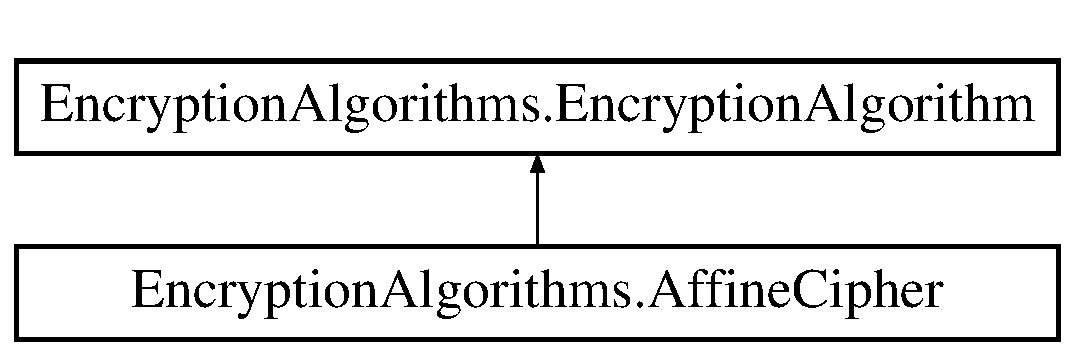
\includegraphics[height=2.000000cm]{classEncryptionAlgorithms_1_1AffineCipher}
\end{center}
\end{figure}
\subsection*{Private Member Functions}
\begin{DoxyCompactItemize}
\item 
def \mbox{\hyperlink{classEncryptionAlgorithms_1_1AffineCipher_afe69f083dfa42c02810e29f80ca04947}{\+\_\+validate\+Key}} (self, key)
\item 
def \mbox{\hyperlink{classEncryptionAlgorithms_1_1AffineCipher_a2904acea89ffc703205906fbb935393d}{\+\_\+validate\+Plain\+Text}} (self, text)
\item 
def \mbox{\hyperlink{classEncryptionAlgorithms_1_1AffineCipher_a6d8229ee69ea1d543f44ac01b16f7413}{\+\_\+validate\+Cipher\+Text}} (self, text)
\item 
def \mbox{\hyperlink{classEncryptionAlgorithms_1_1AffineCipher_ab526a5a15a9d1d616ccb49ff12a37d14}{\+\_\+encrypt}} (self, key, text)
\item 
def \mbox{\hyperlink{classEncryptionAlgorithms_1_1AffineCipher_af29603acbf0ce85d618c8e50ef040604}{\+\_\+decrypt}} (self, key, text)
\end{DoxyCompactItemize}
\subsection*{Additional Inherited Members}


\subsection{Member Function Documentation}
\mbox{\Hypertarget{classEncryptionAlgorithms_1_1AffineCipher_af29603acbf0ce85d618c8e50ef040604}\label{classEncryptionAlgorithms_1_1AffineCipher_af29603acbf0ce85d618c8e50ef040604}} 
\index{Encryption\+Algorithms\+::\+Affine\+Cipher@{Encryption\+Algorithms\+::\+Affine\+Cipher}!\+\_\+decrypt@{\+\_\+decrypt}}
\index{\+\_\+decrypt@{\+\_\+decrypt}!Encryption\+Algorithms\+::\+Affine\+Cipher@{Encryption\+Algorithms\+::\+Affine\+Cipher}}
\subsubsection{\texorpdfstring{\+\_\+decrypt()}{\_decrypt()}}
{\footnotesize\ttfamily def Encryption\+Algorithms.\+Affine\+Cipher.\+\_\+decrypt (\begin{DoxyParamCaption}\item[{}]{self,  }\item[{}]{key,  }\item[{}]{text }\end{DoxyParamCaption})\hspace{0.3cm}{\ttfamily [private]}}

\mbox{\Hypertarget{classEncryptionAlgorithms_1_1AffineCipher_ab526a5a15a9d1d616ccb49ff12a37d14}\label{classEncryptionAlgorithms_1_1AffineCipher_ab526a5a15a9d1d616ccb49ff12a37d14}} 
\index{Encryption\+Algorithms\+::\+Affine\+Cipher@{Encryption\+Algorithms\+::\+Affine\+Cipher}!\+\_\+encrypt@{\+\_\+encrypt}}
\index{\+\_\+encrypt@{\+\_\+encrypt}!Encryption\+Algorithms\+::\+Affine\+Cipher@{Encryption\+Algorithms\+::\+Affine\+Cipher}}
\subsubsection{\texorpdfstring{\+\_\+encrypt()}{\_encrypt()}}
{\footnotesize\ttfamily def Encryption\+Algorithms.\+Affine\+Cipher.\+\_\+encrypt (\begin{DoxyParamCaption}\item[{}]{self,  }\item[{}]{key,  }\item[{}]{text }\end{DoxyParamCaption})\hspace{0.3cm}{\ttfamily [private]}}

\mbox{\Hypertarget{classEncryptionAlgorithms_1_1AffineCipher_a6d8229ee69ea1d543f44ac01b16f7413}\label{classEncryptionAlgorithms_1_1AffineCipher_a6d8229ee69ea1d543f44ac01b16f7413}} 
\index{Encryption\+Algorithms\+::\+Affine\+Cipher@{Encryption\+Algorithms\+::\+Affine\+Cipher}!\+\_\+validate\+Cipher\+Text@{\+\_\+validate\+Cipher\+Text}}
\index{\+\_\+validate\+Cipher\+Text@{\+\_\+validate\+Cipher\+Text}!Encryption\+Algorithms\+::\+Affine\+Cipher@{Encryption\+Algorithms\+::\+Affine\+Cipher}}
\subsubsection{\texorpdfstring{\+\_\+validate\+Cipher\+Text()}{\_validateCipherText()}}
{\footnotesize\ttfamily def Encryption\+Algorithms.\+Affine\+Cipher.\+\_\+validate\+Cipher\+Text (\begin{DoxyParamCaption}\item[{}]{self,  }\item[{}]{text }\end{DoxyParamCaption})\hspace{0.3cm}{\ttfamily [private]}}

\mbox{\Hypertarget{classEncryptionAlgorithms_1_1AffineCipher_afe69f083dfa42c02810e29f80ca04947}\label{classEncryptionAlgorithms_1_1AffineCipher_afe69f083dfa42c02810e29f80ca04947}} 
\index{Encryption\+Algorithms\+::\+Affine\+Cipher@{Encryption\+Algorithms\+::\+Affine\+Cipher}!\+\_\+validate\+Key@{\+\_\+validate\+Key}}
\index{\+\_\+validate\+Key@{\+\_\+validate\+Key}!Encryption\+Algorithms\+::\+Affine\+Cipher@{Encryption\+Algorithms\+::\+Affine\+Cipher}}
\subsubsection{\texorpdfstring{\+\_\+validate\+Key()}{\_validateKey()}}
{\footnotesize\ttfamily def Encryption\+Algorithms.\+Affine\+Cipher.\+\_\+validate\+Key (\begin{DoxyParamCaption}\item[{}]{self,  }\item[{}]{key }\end{DoxyParamCaption})\hspace{0.3cm}{\ttfamily [private]}}

\mbox{\Hypertarget{classEncryptionAlgorithms_1_1AffineCipher_a2904acea89ffc703205906fbb935393d}\label{classEncryptionAlgorithms_1_1AffineCipher_a2904acea89ffc703205906fbb935393d}} 
\index{Encryption\+Algorithms\+::\+Affine\+Cipher@{Encryption\+Algorithms\+::\+Affine\+Cipher}!\+\_\+validate\+Plain\+Text@{\+\_\+validate\+Plain\+Text}}
\index{\+\_\+validate\+Plain\+Text@{\+\_\+validate\+Plain\+Text}!Encryption\+Algorithms\+::\+Affine\+Cipher@{Encryption\+Algorithms\+::\+Affine\+Cipher}}
\subsubsection{\texorpdfstring{\+\_\+validate\+Plain\+Text()}{\_validatePlainText()}}
{\footnotesize\ttfamily def Encryption\+Algorithms.\+Affine\+Cipher.\+\_\+validate\+Plain\+Text (\begin{DoxyParamCaption}\item[{}]{self,  }\item[{}]{text }\end{DoxyParamCaption})\hspace{0.3cm}{\ttfamily [private]}}



The documentation for this class was generated from the following file\+:\begin{DoxyCompactItemize}
\item 
\mbox{\hyperlink{EncryptionAlgorithms_8py}{Encryption\+Algorithms.\+py}}\end{DoxyCompactItemize}

\hypertarget{classEncryptionAlgorithms_1_1BelasoCipher}{}\section{Encryption\+Algorithms.\+Belaso\+Cipher Class Reference}
\label{classEncryptionAlgorithms_1_1BelasoCipher}\index{Encryption\+Algorithms.\+Belaso\+Cipher@{Encryption\+Algorithms.\+Belaso\+Cipher}}
Inheritance diagram for Encryption\+Algorithms.\+Belaso\+Cipher\+:\begin{figure}[H]
\begin{center}
\leavevmode
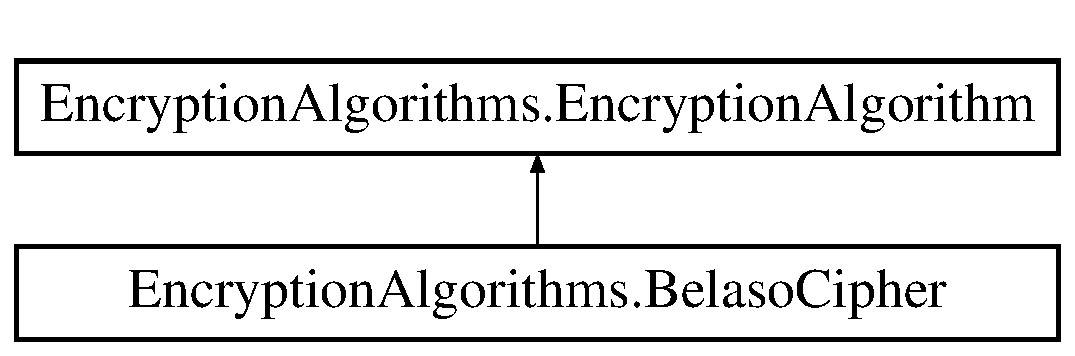
\includegraphics[height=2.000000cm]{classEncryptionAlgorithms_1_1BelasoCipher}
\end{center}
\end{figure}
\subsection*{Private Member Functions}
\begin{DoxyCompactItemize}
\item 
def \mbox{\hyperlink{classEncryptionAlgorithms_1_1BelasoCipher_a3a22e598ed13e45113525b83f21edc39}{\+\_\+validate\+Key}} (self, key)
\item 
def \mbox{\hyperlink{classEncryptionAlgorithms_1_1BelasoCipher_ae1a862a944f83bcfd1a69548d0127025}{\+\_\+validate\+Plain\+Text}} (self, text)
\item 
def \mbox{\hyperlink{classEncryptionAlgorithms_1_1BelasoCipher_a27be6c3ef5ece5d4f7f2c07bd6018c22}{\+\_\+validate\+Cipher\+Text}} (self, text)
\item 
def \mbox{\hyperlink{classEncryptionAlgorithms_1_1BelasoCipher_ae7294f9e4900ceafbdcc4bd2c855a7e9}{\+\_\+encrypt}} (self, key, text)
\item 
def \mbox{\hyperlink{classEncryptionAlgorithms_1_1BelasoCipher_a65864039ed30946238a13105f8d53bde}{\+\_\+decrypt}} (self, key, text)
\end{DoxyCompactItemize}
\subsection*{Additional Inherited Members}


\subsection{Member Function Documentation}
\mbox{\Hypertarget{classEncryptionAlgorithms_1_1BelasoCipher_a65864039ed30946238a13105f8d53bde}\label{classEncryptionAlgorithms_1_1BelasoCipher_a65864039ed30946238a13105f8d53bde}} 
\index{Encryption\+Algorithms\+::\+Belaso\+Cipher@{Encryption\+Algorithms\+::\+Belaso\+Cipher}!\+\_\+decrypt@{\+\_\+decrypt}}
\index{\+\_\+decrypt@{\+\_\+decrypt}!Encryption\+Algorithms\+::\+Belaso\+Cipher@{Encryption\+Algorithms\+::\+Belaso\+Cipher}}
\subsubsection{\texorpdfstring{\+\_\+decrypt()}{\_decrypt()}}
{\footnotesize\ttfamily def Encryption\+Algorithms.\+Belaso\+Cipher.\+\_\+decrypt (\begin{DoxyParamCaption}\item[{}]{self,  }\item[{}]{key,  }\item[{}]{text }\end{DoxyParamCaption})\hspace{0.3cm}{\ttfamily [private]}}

\mbox{\Hypertarget{classEncryptionAlgorithms_1_1BelasoCipher_ae7294f9e4900ceafbdcc4bd2c855a7e9}\label{classEncryptionAlgorithms_1_1BelasoCipher_ae7294f9e4900ceafbdcc4bd2c855a7e9}} 
\index{Encryption\+Algorithms\+::\+Belaso\+Cipher@{Encryption\+Algorithms\+::\+Belaso\+Cipher}!\+\_\+encrypt@{\+\_\+encrypt}}
\index{\+\_\+encrypt@{\+\_\+encrypt}!Encryption\+Algorithms\+::\+Belaso\+Cipher@{Encryption\+Algorithms\+::\+Belaso\+Cipher}}
\subsubsection{\texorpdfstring{\+\_\+encrypt()}{\_encrypt()}}
{\footnotesize\ttfamily def Encryption\+Algorithms.\+Belaso\+Cipher.\+\_\+encrypt (\begin{DoxyParamCaption}\item[{}]{self,  }\item[{}]{key,  }\item[{}]{text }\end{DoxyParamCaption})\hspace{0.3cm}{\ttfamily [private]}}

\mbox{\Hypertarget{classEncryptionAlgorithms_1_1BelasoCipher_a27be6c3ef5ece5d4f7f2c07bd6018c22}\label{classEncryptionAlgorithms_1_1BelasoCipher_a27be6c3ef5ece5d4f7f2c07bd6018c22}} 
\index{Encryption\+Algorithms\+::\+Belaso\+Cipher@{Encryption\+Algorithms\+::\+Belaso\+Cipher}!\+\_\+validate\+Cipher\+Text@{\+\_\+validate\+Cipher\+Text}}
\index{\+\_\+validate\+Cipher\+Text@{\+\_\+validate\+Cipher\+Text}!Encryption\+Algorithms\+::\+Belaso\+Cipher@{Encryption\+Algorithms\+::\+Belaso\+Cipher}}
\subsubsection{\texorpdfstring{\+\_\+validate\+Cipher\+Text()}{\_validateCipherText()}}
{\footnotesize\ttfamily def Encryption\+Algorithms.\+Belaso\+Cipher.\+\_\+validate\+Cipher\+Text (\begin{DoxyParamCaption}\item[{}]{self,  }\item[{}]{text }\end{DoxyParamCaption})\hspace{0.3cm}{\ttfamily [private]}}

\mbox{\Hypertarget{classEncryptionAlgorithms_1_1BelasoCipher_a3a22e598ed13e45113525b83f21edc39}\label{classEncryptionAlgorithms_1_1BelasoCipher_a3a22e598ed13e45113525b83f21edc39}} 
\index{Encryption\+Algorithms\+::\+Belaso\+Cipher@{Encryption\+Algorithms\+::\+Belaso\+Cipher}!\+\_\+validate\+Key@{\+\_\+validate\+Key}}
\index{\+\_\+validate\+Key@{\+\_\+validate\+Key}!Encryption\+Algorithms\+::\+Belaso\+Cipher@{Encryption\+Algorithms\+::\+Belaso\+Cipher}}
\subsubsection{\texorpdfstring{\+\_\+validate\+Key()}{\_validateKey()}}
{\footnotesize\ttfamily def Encryption\+Algorithms.\+Belaso\+Cipher.\+\_\+validate\+Key (\begin{DoxyParamCaption}\item[{}]{self,  }\item[{}]{key }\end{DoxyParamCaption})\hspace{0.3cm}{\ttfamily [private]}}

\mbox{\Hypertarget{classEncryptionAlgorithms_1_1BelasoCipher_ae1a862a944f83bcfd1a69548d0127025}\label{classEncryptionAlgorithms_1_1BelasoCipher_ae1a862a944f83bcfd1a69548d0127025}} 
\index{Encryption\+Algorithms\+::\+Belaso\+Cipher@{Encryption\+Algorithms\+::\+Belaso\+Cipher}!\+\_\+validate\+Plain\+Text@{\+\_\+validate\+Plain\+Text}}
\index{\+\_\+validate\+Plain\+Text@{\+\_\+validate\+Plain\+Text}!Encryption\+Algorithms\+::\+Belaso\+Cipher@{Encryption\+Algorithms\+::\+Belaso\+Cipher}}
\subsubsection{\texorpdfstring{\+\_\+validate\+Plain\+Text()}{\_validatePlainText()}}
{\footnotesize\ttfamily def Encryption\+Algorithms.\+Belaso\+Cipher.\+\_\+validate\+Plain\+Text (\begin{DoxyParamCaption}\item[{}]{self,  }\item[{}]{text }\end{DoxyParamCaption})\hspace{0.3cm}{\ttfamily [private]}}



The documentation for this class was generated from the following file\+:\begin{DoxyCompactItemize}
\item 
\mbox{\hyperlink{EncryptionAlgorithms_8py}{Encryption\+Algorithms.\+py}}\end{DoxyCompactItemize}

\hypertarget{classEncryptionAlgorithms_1_1CaesarCipher}{}\section{Encryption\+Algorithms.\+Caesar\+Cipher Class Reference}
\label{classEncryptionAlgorithms_1_1CaesarCipher}\index{Encryption\+Algorithms.\+Caesar\+Cipher@{Encryption\+Algorithms.\+Caesar\+Cipher}}


Implements the Caesar cipher, has all methods from \mbox{\hyperlink{classEncryptionAlgorithms_1_1EncryptionAlgorithm}{Encryption\+Algorithm}}.  


Inheritance diagram for Encryption\+Algorithms.\+Caesar\+Cipher\+:\begin{figure}[H]
\begin{center}
\leavevmode
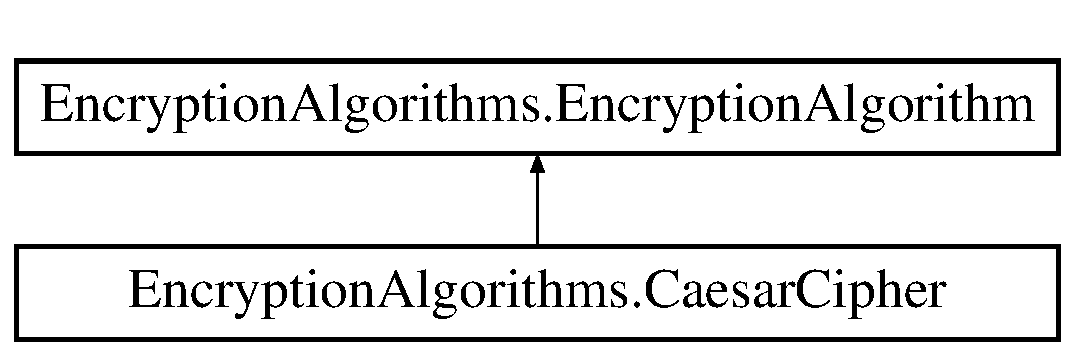
\includegraphics[height=2.000000cm]{classEncryptionAlgorithms_1_1CaesarCipher}
\end{center}
\end{figure}
\subsection*{Private Member Functions}
\begin{DoxyCompactItemize}
\item 
def \mbox{\hyperlink{classEncryptionAlgorithms_1_1CaesarCipher_af790e8acc754ab66e19652aaf003ef45}{\+\_\+validate\+Key}} (self, key)
\begin{DoxyCompactList}\small\item\em validates the key. \end{DoxyCompactList}\item 
def \mbox{\hyperlink{classEncryptionAlgorithms_1_1CaesarCipher_a6fe0acdce6b92624ba362c1b14a06e2b}{\+\_\+validate\+Plain\+Text}} (self, text)
\begin{DoxyCompactList}\small\item\em validates the plain text. \end{DoxyCompactList}\item 
def \mbox{\hyperlink{classEncryptionAlgorithms_1_1CaesarCipher_a55a7fb968fe4d734b8692271bba17c6b}{\+\_\+validate\+Cipher\+Text}} (self, text)
\begin{DoxyCompactList}\small\item\em validates the cipher text. \end{DoxyCompactList}\item 
def \mbox{\hyperlink{classEncryptionAlgorithms_1_1CaesarCipher_aa9613b0dd8ed0a3331a12ce3b607940b}{\+\_\+encrypt}} (self, key, text)
\begin{DoxyCompactList}\small\item\em Internal encryption function. \end{DoxyCompactList}\item 
def \mbox{\hyperlink{classEncryptionAlgorithms_1_1CaesarCipher_a26694e19444bbcb58987f24205cdbce7}{\+\_\+decrypt}} (self, key, text)
\begin{DoxyCompactList}\small\item\em Internal decryption function. \end{DoxyCompactList}\end{DoxyCompactItemize}
\subsection*{Additional Inherited Members}


\subsection{Detailed Description}
Implements the Caesar cipher, has all methods from \mbox{\hyperlink{classEncryptionAlgorithms_1_1EncryptionAlgorithm}{Encryption\+Algorithm}}. 

\subsection{Member Function Documentation}
\mbox{\Hypertarget{classEncryptionAlgorithms_1_1CaesarCipher_a26694e19444bbcb58987f24205cdbce7}\label{classEncryptionAlgorithms_1_1CaesarCipher_a26694e19444bbcb58987f24205cdbce7}} 
\index{Encryption\+Algorithms\+::\+Caesar\+Cipher@{Encryption\+Algorithms\+::\+Caesar\+Cipher}!\+\_\+decrypt@{\+\_\+decrypt}}
\index{\+\_\+decrypt@{\+\_\+decrypt}!Encryption\+Algorithms\+::\+Caesar\+Cipher@{Encryption\+Algorithms\+::\+Caesar\+Cipher}}
\subsubsection{\texorpdfstring{\+\_\+decrypt()}{\_decrypt()}}
{\footnotesize\ttfamily def Encryption\+Algorithms.\+Caesar\+Cipher.\+\_\+decrypt (\begin{DoxyParamCaption}\item[{}]{self,  }\item[{}]{key,  }\item[{}]{text }\end{DoxyParamCaption})\hspace{0.3cm}{\ttfamily [private]}}



Internal decryption function. 

Encrypth with -\/key


\begin{DoxyParams}{Parameters}
{\em key} & \\
\hline
{\em text} & \\
\hline
\end{DoxyParams}
\begin{DoxyReturn}{Returns}

\end{DoxyReturn}
\mbox{\Hypertarget{classEncryptionAlgorithms_1_1CaesarCipher_aa9613b0dd8ed0a3331a12ce3b607940b}\label{classEncryptionAlgorithms_1_1CaesarCipher_aa9613b0dd8ed0a3331a12ce3b607940b}} 
\index{Encryption\+Algorithms\+::\+Caesar\+Cipher@{Encryption\+Algorithms\+::\+Caesar\+Cipher}!\+\_\+encrypt@{\+\_\+encrypt}}
\index{\+\_\+encrypt@{\+\_\+encrypt}!Encryption\+Algorithms\+::\+Caesar\+Cipher@{Encryption\+Algorithms\+::\+Caesar\+Cipher}}
\subsubsection{\texorpdfstring{\+\_\+encrypt()}{\_encrypt()}}
{\footnotesize\ttfamily def Encryption\+Algorithms.\+Caesar\+Cipher.\+\_\+encrypt (\begin{DoxyParamCaption}\item[{}]{self,  }\item[{}]{key,  }\item[{}]{text }\end{DoxyParamCaption})\hspace{0.3cm}{\ttfamily [private]}}



Internal encryption function. 

Shifts each character from the plaintext by \textquotesingle{}key\textquotesingle{} ammount of characters in the alphabet.


\begin{DoxyParams}{Parameters}
{\em key} & \\
\hline
{\em text} & \\
\hline
\end{DoxyParams}
\begin{DoxyReturn}{Returns}

\end{DoxyReturn}
\mbox{\Hypertarget{classEncryptionAlgorithms_1_1CaesarCipher_a55a7fb968fe4d734b8692271bba17c6b}\label{classEncryptionAlgorithms_1_1CaesarCipher_a55a7fb968fe4d734b8692271bba17c6b}} 
\index{Encryption\+Algorithms\+::\+Caesar\+Cipher@{Encryption\+Algorithms\+::\+Caesar\+Cipher}!\+\_\+validate\+Cipher\+Text@{\+\_\+validate\+Cipher\+Text}}
\index{\+\_\+validate\+Cipher\+Text@{\+\_\+validate\+Cipher\+Text}!Encryption\+Algorithms\+::\+Caesar\+Cipher@{Encryption\+Algorithms\+::\+Caesar\+Cipher}}
\subsubsection{\texorpdfstring{\+\_\+validate\+Cipher\+Text()}{\_validateCipherText()}}
{\footnotesize\ttfamily def Encryption\+Algorithms.\+Caesar\+Cipher.\+\_\+validate\+Cipher\+Text (\begin{DoxyParamCaption}\item[{}]{self,  }\item[{}]{text }\end{DoxyParamCaption})\hspace{0.3cm}{\ttfamily [private]}}



validates the cipher text. 

Throws Validation\+Exception. Ciphertext has to contain only characters from the uppercase(alphabet).


\begin{DoxyParams}{Parameters}
{\em text} & \\
\hline
\end{DoxyParams}
\begin{DoxyReturn}{Returns}

\end{DoxyReturn}
\mbox{\Hypertarget{classEncryptionAlgorithms_1_1CaesarCipher_af790e8acc754ab66e19652aaf003ef45}\label{classEncryptionAlgorithms_1_1CaesarCipher_af790e8acc754ab66e19652aaf003ef45}} 
\index{Encryption\+Algorithms\+::\+Caesar\+Cipher@{Encryption\+Algorithms\+::\+Caesar\+Cipher}!\+\_\+validate\+Key@{\+\_\+validate\+Key}}
\index{\+\_\+validate\+Key@{\+\_\+validate\+Key}!Encryption\+Algorithms\+::\+Caesar\+Cipher@{Encryption\+Algorithms\+::\+Caesar\+Cipher}}
\subsubsection{\texorpdfstring{\+\_\+validate\+Key()}{\_validateKey()}}
{\footnotesize\ttfamily def Encryption\+Algorithms.\+Caesar\+Cipher.\+\_\+validate\+Key (\begin{DoxyParamCaption}\item[{}]{self,  }\item[{}]{key }\end{DoxyParamCaption})\hspace{0.3cm}{\ttfamily [private]}}



validates the key. 

Throws Validation\+Exception. Key has to be an integer between 0 and alphabet length.


\begin{DoxyParams}{Parameters}
{\em key} & \\
\hline
\end{DoxyParams}
\begin{DoxyReturn}{Returns}

\end{DoxyReturn}
\mbox{\Hypertarget{classEncryptionAlgorithms_1_1CaesarCipher_a6fe0acdce6b92624ba362c1b14a06e2b}\label{classEncryptionAlgorithms_1_1CaesarCipher_a6fe0acdce6b92624ba362c1b14a06e2b}} 
\index{Encryption\+Algorithms\+::\+Caesar\+Cipher@{Encryption\+Algorithms\+::\+Caesar\+Cipher}!\+\_\+validate\+Plain\+Text@{\+\_\+validate\+Plain\+Text}}
\index{\+\_\+validate\+Plain\+Text@{\+\_\+validate\+Plain\+Text}!Encryption\+Algorithms\+::\+Caesar\+Cipher@{Encryption\+Algorithms\+::\+Caesar\+Cipher}}
\subsubsection{\texorpdfstring{\+\_\+validate\+Plain\+Text()}{\_validatePlainText()}}
{\footnotesize\ttfamily def Encryption\+Algorithms.\+Caesar\+Cipher.\+\_\+validate\+Plain\+Text (\begin{DoxyParamCaption}\item[{}]{self,  }\item[{}]{text }\end{DoxyParamCaption})\hspace{0.3cm}{\ttfamily [private]}}



validates the plain text. 

Throws Validation\+Exception. Plaintext has to contain only characters from the alphabet.


\begin{DoxyParams}{Parameters}
{\em text} & \\
\hline
\end{DoxyParams}
\begin{DoxyReturn}{Returns}

\end{DoxyReturn}


The documentation for this class was generated from the following file\+:\begin{DoxyCompactItemize}
\item 
\mbox{\hyperlink{EncryptionAlgorithms_8py}{Encryption\+Algorithms.\+py}}\end{DoxyCompactItemize}

\hypertarget{classEncryptionAlgorithms_1_1EncryptionAlgorithm}{}\section{Encryption\+Algorithms.\+Encryption\+Algorithm Class Reference}
\label{classEncryptionAlgorithms_1_1EncryptionAlgorithm}\index{Encryption\+Algorithms.\+Encryption\+Algorithm@{Encryption\+Algorithms.\+Encryption\+Algorithm}}


Base encryption algorigm class, defines the A\+PI.  


Inheritance diagram for Encryption\+Algorithms.\+Encryption\+Algorithm\+:\begin{figure}[H]
\begin{center}
\leavevmode
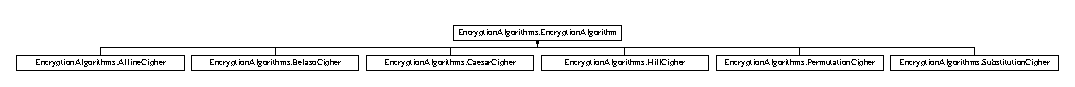
\includegraphics[height=0.723514cm]{classEncryptionAlgorithms_1_1EncryptionAlgorithm}
\end{center}
\end{figure}
\subsection*{Public Member Functions}
\begin{DoxyCompactItemize}
\item 
def \mbox{\hyperlink{classEncryptionAlgorithms_1_1EncryptionAlgorithm_a8916994ba410f389e2cdfd5d77c2d8fa}{\+\_\+\+\_\+init\+\_\+\+\_\+}} (self, \mbox{\hyperlink{classEncryptionAlgorithms_1_1EncryptionAlgorithm_ad43b0d5680d18b7bc62848864e496684}{alphabet}})
\begin{DoxyCompactList}\small\item\em Constructor. \end{DoxyCompactList}\item 
def \mbox{\hyperlink{classEncryptionAlgorithms_1_1EncryptionAlgorithm_af584e5bbf78770ca1d8f8c08c06e0dc2}{set\+Alphabet}} (self, \mbox{\hyperlink{classEncryptionAlgorithms_1_1EncryptionAlgorithm_ad43b0d5680d18b7bc62848864e496684}{alphabet}})
\begin{DoxyCompactList}\small\item\em Sets the new alphabet, validates it. \end{DoxyCompactList}\item 
def \mbox{\hyperlink{classEncryptionAlgorithms_1_1EncryptionAlgorithm_ac8e6b3a5b536ba2b3ed86f4f635be679}{encrypt}} (self, key, text)
\begin{DoxyCompactList}\small\item\em Encryption function, validates key and plaintext. \end{DoxyCompactList}\item 
def \mbox{\hyperlink{classEncryptionAlgorithms_1_1EncryptionAlgorithm_ab0666e938c8fbcce0934f145288397d9}{decrypt}} (self, key, text)
\begin{DoxyCompactList}\small\item\em Decryption function, validates key and ciphertext. \end{DoxyCompactList}\end{DoxyCompactItemize}
\subsection*{Public Attributes}
\begin{DoxyCompactItemize}
\item 
\mbox{\hyperlink{classEncryptionAlgorithms_1_1EncryptionAlgorithm_ad43b0d5680d18b7bc62848864e496684}{alphabet}}
\end{DoxyCompactItemize}
\subsection*{Private Member Functions}
\begin{DoxyCompactItemize}
\item 
def \mbox{\hyperlink{classEncryptionAlgorithms_1_1EncryptionAlgorithm_af3d6de15270153827e6928c5e9fd65be}{\+\_\+validate\+Alphabet}} (self, \mbox{\hyperlink{classEncryptionAlgorithms_1_1EncryptionAlgorithm_ad43b0d5680d18b7bc62848864e496684}{alphabet}})
\begin{DoxyCompactList}\small\item\em internal method for validating the alphabet \end{DoxyCompactList}\item 
def \mbox{\hyperlink{classEncryptionAlgorithms_1_1EncryptionAlgorithm_af28e6d27846bd1690122b68edb95a486}{\+\_\+validate\+Key}} (self, key)
\begin{DoxyCompactList}\small\item\em Validates the key. \end{DoxyCompactList}\item 
def \mbox{\hyperlink{classEncryptionAlgorithms_1_1EncryptionAlgorithm_a78d73cf66cbaca8f534bbfd5609a984d}{\+\_\+validate\+Plain\+Text}} (self, text)
\begin{DoxyCompactList}\small\item\em validates the plain text. \end{DoxyCompactList}\item 
def \mbox{\hyperlink{classEncryptionAlgorithms_1_1EncryptionAlgorithm_a1b5077d40cae2bb5d71e9a7df94757c4}{\+\_\+validate\+Cipher\+Text}} (self, text)
\begin{DoxyCompactList}\small\item\em validates the cipher text. \end{DoxyCompactList}\item 
def \mbox{\hyperlink{classEncryptionAlgorithms_1_1EncryptionAlgorithm_ab69e2900b19527168901b083b4eb4ec4}{\+\_\+encrypt}} (self, key, text)
\begin{DoxyCompactList}\small\item\em internal encryption function, called by encrypt \end{DoxyCompactList}\item 
def \mbox{\hyperlink{classEncryptionAlgorithms_1_1EncryptionAlgorithm_af2c4a5b86561ddb3d9465477b83904b5}{\+\_\+decrypt}} (self, key, text)
\begin{DoxyCompactList}\small\item\em internal decryption function, called by decrypt \end{DoxyCompactList}\end{DoxyCompactItemize}


\subsection{Detailed Description}
Base encryption algorigm class, defines the A\+PI. 

\subsection{Constructor \& Destructor Documentation}
\mbox{\Hypertarget{classEncryptionAlgorithms_1_1EncryptionAlgorithm_a8916994ba410f389e2cdfd5d77c2d8fa}\label{classEncryptionAlgorithms_1_1EncryptionAlgorithm_a8916994ba410f389e2cdfd5d77c2d8fa}} 
\index{Encryption\+Algorithms\+::\+Encryption\+Algorithm@{Encryption\+Algorithms\+::\+Encryption\+Algorithm}!\+\_\+\+\_\+init\+\_\+\+\_\+@{\+\_\+\+\_\+init\+\_\+\+\_\+}}
\index{\+\_\+\+\_\+init\+\_\+\+\_\+@{\+\_\+\+\_\+init\+\_\+\+\_\+}!Encryption\+Algorithms\+::\+Encryption\+Algorithm@{Encryption\+Algorithms\+::\+Encryption\+Algorithm}}
\subsubsection{\texorpdfstring{\+\_\+\+\_\+init\+\_\+\+\_\+()}{\_\_init\_\_()}}
{\footnotesize\ttfamily def Encryption\+Algorithms.\+Encryption\+Algorithm.\+\_\+\+\_\+init\+\_\+\+\_\+ (\begin{DoxyParamCaption}\item[{}]{self,  }\item[{}]{alphabet }\end{DoxyParamCaption})}



Constructor. 


\begin{DoxyParams}{Parameters}
{\em alphabet} & string -\/ List of symbols for plaintext and ciphertext\\
\hline
\end{DoxyParams}
\begin{DoxyReturn}{Returns}
The object 
\end{DoxyReturn}


\subsection{Member Function Documentation}
\mbox{\Hypertarget{classEncryptionAlgorithms_1_1EncryptionAlgorithm_af2c4a5b86561ddb3d9465477b83904b5}\label{classEncryptionAlgorithms_1_1EncryptionAlgorithm_af2c4a5b86561ddb3d9465477b83904b5}} 
\index{Encryption\+Algorithms\+::\+Encryption\+Algorithm@{Encryption\+Algorithms\+::\+Encryption\+Algorithm}!\+\_\+decrypt@{\+\_\+decrypt}}
\index{\+\_\+decrypt@{\+\_\+decrypt}!Encryption\+Algorithms\+::\+Encryption\+Algorithm@{Encryption\+Algorithms\+::\+Encryption\+Algorithm}}
\subsubsection{\texorpdfstring{\+\_\+decrypt()}{\_decrypt()}}
{\footnotesize\ttfamily def Encryption\+Algorithms.\+Encryption\+Algorithm.\+\_\+decrypt (\begin{DoxyParamCaption}\item[{}]{self,  }\item[{}]{key,  }\item[{}]{text }\end{DoxyParamCaption})\hspace{0.3cm}{\ttfamily [private]}}



internal decryption function, called by decrypt 


\begin{DoxyParams}{Parameters}
{\em key} & \\
\hline
{\em text} & \\
\hline
\end{DoxyParams}
\begin{DoxyReturn}{Returns}
decrypted text 
\end{DoxyReturn}
\mbox{\Hypertarget{classEncryptionAlgorithms_1_1EncryptionAlgorithm_ab69e2900b19527168901b083b4eb4ec4}\label{classEncryptionAlgorithms_1_1EncryptionAlgorithm_ab69e2900b19527168901b083b4eb4ec4}} 
\index{Encryption\+Algorithms\+::\+Encryption\+Algorithm@{Encryption\+Algorithms\+::\+Encryption\+Algorithm}!\+\_\+encrypt@{\+\_\+encrypt}}
\index{\+\_\+encrypt@{\+\_\+encrypt}!Encryption\+Algorithms\+::\+Encryption\+Algorithm@{Encryption\+Algorithms\+::\+Encryption\+Algorithm}}
\subsubsection{\texorpdfstring{\+\_\+encrypt()}{\_encrypt()}}
{\footnotesize\ttfamily def Encryption\+Algorithms.\+Encryption\+Algorithm.\+\_\+encrypt (\begin{DoxyParamCaption}\item[{}]{self,  }\item[{}]{key,  }\item[{}]{text }\end{DoxyParamCaption})\hspace{0.3cm}{\ttfamily [private]}}



internal encryption function, called by encrypt 


\begin{DoxyParams}{Parameters}
{\em key} & \\
\hline
{\em text} & \\
\hline
\end{DoxyParams}
\begin{DoxyReturn}{Returns}
encrypted text 
\end{DoxyReturn}
\mbox{\Hypertarget{classEncryptionAlgorithms_1_1EncryptionAlgorithm_af3d6de15270153827e6928c5e9fd65be}\label{classEncryptionAlgorithms_1_1EncryptionAlgorithm_af3d6de15270153827e6928c5e9fd65be}} 
\index{Encryption\+Algorithms\+::\+Encryption\+Algorithm@{Encryption\+Algorithms\+::\+Encryption\+Algorithm}!\+\_\+validate\+Alphabet@{\+\_\+validate\+Alphabet}}
\index{\+\_\+validate\+Alphabet@{\+\_\+validate\+Alphabet}!Encryption\+Algorithms\+::\+Encryption\+Algorithm@{Encryption\+Algorithms\+::\+Encryption\+Algorithm}}
\subsubsection{\texorpdfstring{\+\_\+validate\+Alphabet()}{\_validateAlphabet()}}
{\footnotesize\ttfamily def Encryption\+Algorithms.\+Encryption\+Algorithm.\+\_\+validate\+Alphabet (\begin{DoxyParamCaption}\item[{}]{self,  }\item[{}]{alphabet }\end{DoxyParamCaption})\hspace{0.3cm}{\ttfamily [private]}}



internal method for validating the alphabet 


\begin{DoxyParams}{Parameters}
{\em alphabet} & \\
\hline
\end{DoxyParams}
\begin{DoxyReturn}{Returns}

\end{DoxyReturn}
\mbox{\Hypertarget{classEncryptionAlgorithms_1_1EncryptionAlgorithm_a1b5077d40cae2bb5d71e9a7df94757c4}\label{classEncryptionAlgorithms_1_1EncryptionAlgorithm_a1b5077d40cae2bb5d71e9a7df94757c4}} 
\index{Encryption\+Algorithms\+::\+Encryption\+Algorithm@{Encryption\+Algorithms\+::\+Encryption\+Algorithm}!\+\_\+validate\+Cipher\+Text@{\+\_\+validate\+Cipher\+Text}}
\index{\+\_\+validate\+Cipher\+Text@{\+\_\+validate\+Cipher\+Text}!Encryption\+Algorithms\+::\+Encryption\+Algorithm@{Encryption\+Algorithms\+::\+Encryption\+Algorithm}}
\subsubsection{\texorpdfstring{\+\_\+validate\+Cipher\+Text()}{\_validateCipherText()}}
{\footnotesize\ttfamily def Encryption\+Algorithms.\+Encryption\+Algorithm.\+\_\+validate\+Cipher\+Text (\begin{DoxyParamCaption}\item[{}]{self,  }\item[{}]{text }\end{DoxyParamCaption})\hspace{0.3cm}{\ttfamily [private]}}



validates the cipher text. 

Throws Validation\+Exception


\begin{DoxyParams}{Parameters}
{\em text} & \\
\hline
\end{DoxyParams}
\begin{DoxyReturn}{Returns}

\end{DoxyReturn}
\mbox{\Hypertarget{classEncryptionAlgorithms_1_1EncryptionAlgorithm_af28e6d27846bd1690122b68edb95a486}\label{classEncryptionAlgorithms_1_1EncryptionAlgorithm_af28e6d27846bd1690122b68edb95a486}} 
\index{Encryption\+Algorithms\+::\+Encryption\+Algorithm@{Encryption\+Algorithms\+::\+Encryption\+Algorithm}!\+\_\+validate\+Key@{\+\_\+validate\+Key}}
\index{\+\_\+validate\+Key@{\+\_\+validate\+Key}!Encryption\+Algorithms\+::\+Encryption\+Algorithm@{Encryption\+Algorithms\+::\+Encryption\+Algorithm}}
\subsubsection{\texorpdfstring{\+\_\+validate\+Key()}{\_validateKey()}}
{\footnotesize\ttfamily def Encryption\+Algorithms.\+Encryption\+Algorithm.\+\_\+validate\+Key (\begin{DoxyParamCaption}\item[{}]{self,  }\item[{}]{key }\end{DoxyParamCaption})\hspace{0.3cm}{\ttfamily [private]}}



Validates the key. 

Throws Validation\+Exception


\begin{DoxyParams}{Parameters}
{\em key} & \\
\hline
\end{DoxyParams}
\begin{DoxyReturn}{Returns}
None 
\end{DoxyReturn}
\mbox{\Hypertarget{classEncryptionAlgorithms_1_1EncryptionAlgorithm_a78d73cf66cbaca8f534bbfd5609a984d}\label{classEncryptionAlgorithms_1_1EncryptionAlgorithm_a78d73cf66cbaca8f534bbfd5609a984d}} 
\index{Encryption\+Algorithms\+::\+Encryption\+Algorithm@{Encryption\+Algorithms\+::\+Encryption\+Algorithm}!\+\_\+validate\+Plain\+Text@{\+\_\+validate\+Plain\+Text}}
\index{\+\_\+validate\+Plain\+Text@{\+\_\+validate\+Plain\+Text}!Encryption\+Algorithms\+::\+Encryption\+Algorithm@{Encryption\+Algorithms\+::\+Encryption\+Algorithm}}
\subsubsection{\texorpdfstring{\+\_\+validate\+Plain\+Text()}{\_validatePlainText()}}
{\footnotesize\ttfamily def Encryption\+Algorithms.\+Encryption\+Algorithm.\+\_\+validate\+Plain\+Text (\begin{DoxyParamCaption}\item[{}]{self,  }\item[{}]{text }\end{DoxyParamCaption})\hspace{0.3cm}{\ttfamily [private]}}



validates the plain text. 

Throws Validation\+Exception


\begin{DoxyParams}{Parameters}
{\em text} & \\
\hline
\end{DoxyParams}
\begin{DoxyReturn}{Returns}

\end{DoxyReturn}
\mbox{\Hypertarget{classEncryptionAlgorithms_1_1EncryptionAlgorithm_ab0666e938c8fbcce0934f145288397d9}\label{classEncryptionAlgorithms_1_1EncryptionAlgorithm_ab0666e938c8fbcce0934f145288397d9}} 
\index{Encryption\+Algorithms\+::\+Encryption\+Algorithm@{Encryption\+Algorithms\+::\+Encryption\+Algorithm}!decrypt@{decrypt}}
\index{decrypt@{decrypt}!Encryption\+Algorithms\+::\+Encryption\+Algorithm@{Encryption\+Algorithms\+::\+Encryption\+Algorithm}}
\subsubsection{\texorpdfstring{decrypt()}{decrypt()}}
{\footnotesize\ttfamily def Encryption\+Algorithms.\+Encryption\+Algorithm.\+decrypt (\begin{DoxyParamCaption}\item[{}]{self,  }\item[{}]{key,  }\item[{}]{text }\end{DoxyParamCaption})}



Decryption function, validates key and ciphertext. 


\begin{DoxyParams}{Parameters}
{\em key} & \\
\hline
{\em text} & \\
\hline
\end{DoxyParams}
\begin{DoxyReturn}{Returns}
Decrypted text 
\end{DoxyReturn}
\mbox{\Hypertarget{classEncryptionAlgorithms_1_1EncryptionAlgorithm_ac8e6b3a5b536ba2b3ed86f4f635be679}\label{classEncryptionAlgorithms_1_1EncryptionAlgorithm_ac8e6b3a5b536ba2b3ed86f4f635be679}} 
\index{Encryption\+Algorithms\+::\+Encryption\+Algorithm@{Encryption\+Algorithms\+::\+Encryption\+Algorithm}!encrypt@{encrypt}}
\index{encrypt@{encrypt}!Encryption\+Algorithms\+::\+Encryption\+Algorithm@{Encryption\+Algorithms\+::\+Encryption\+Algorithm}}
\subsubsection{\texorpdfstring{encrypt()}{encrypt()}}
{\footnotesize\ttfamily def Encryption\+Algorithms.\+Encryption\+Algorithm.\+encrypt (\begin{DoxyParamCaption}\item[{}]{self,  }\item[{}]{key,  }\item[{}]{text }\end{DoxyParamCaption})}



Encryption function, validates key and plaintext. 

Throws Validation\+Exception


\begin{DoxyParams}{Parameters}
{\em key} & \\
\hline
{\em text} & \\
\hline
\end{DoxyParams}
\begin{DoxyReturn}{Returns}
Encrypted text 
\end{DoxyReturn}
\mbox{\Hypertarget{classEncryptionAlgorithms_1_1EncryptionAlgorithm_af584e5bbf78770ca1d8f8c08c06e0dc2}\label{classEncryptionAlgorithms_1_1EncryptionAlgorithm_af584e5bbf78770ca1d8f8c08c06e0dc2}} 
\index{Encryption\+Algorithms\+::\+Encryption\+Algorithm@{Encryption\+Algorithms\+::\+Encryption\+Algorithm}!set\+Alphabet@{set\+Alphabet}}
\index{set\+Alphabet@{set\+Alphabet}!Encryption\+Algorithms\+::\+Encryption\+Algorithm@{Encryption\+Algorithms\+::\+Encryption\+Algorithm}}
\subsubsection{\texorpdfstring{set\+Alphabet()}{setAlphabet()}}
{\footnotesize\ttfamily def Encryption\+Algorithms.\+Encryption\+Algorithm.\+set\+Alphabet (\begin{DoxyParamCaption}\item[{}]{self,  }\item[{}]{alphabet }\end{DoxyParamCaption})}



Sets the new alphabet, validates it. 


\begin{DoxyParams}{Parameters}
{\em alphabet} & -\/ string\\
\hline
\end{DoxyParams}
\begin{DoxyReturn}{Returns}
None 
\end{DoxyReturn}


\subsection{Member Data Documentation}
\mbox{\Hypertarget{classEncryptionAlgorithms_1_1EncryptionAlgorithm_ad43b0d5680d18b7bc62848864e496684}\label{classEncryptionAlgorithms_1_1EncryptionAlgorithm_ad43b0d5680d18b7bc62848864e496684}} 
\index{Encryption\+Algorithms\+::\+Encryption\+Algorithm@{Encryption\+Algorithms\+::\+Encryption\+Algorithm}!alphabet@{alphabet}}
\index{alphabet@{alphabet}!Encryption\+Algorithms\+::\+Encryption\+Algorithm@{Encryption\+Algorithms\+::\+Encryption\+Algorithm}}
\subsubsection{\texorpdfstring{alphabet}{alphabet}}
{\footnotesize\ttfamily Encryption\+Algorithms.\+Encryption\+Algorithm.\+alphabet}



The documentation for this class was generated from the following file\+:\begin{DoxyCompactItemize}
\item 
\mbox{\hyperlink{EncryptionAlgorithms_8py}{Encryption\+Algorithms.\+py}}\end{DoxyCompactItemize}

\hypertarget{classEncryptionAlgorithms_1_1HillCipher}{}\section{Encryption\+Algorithms.\+Hill\+Cipher Class Reference}
\label{classEncryptionAlgorithms_1_1HillCipher}\index{Encryption\+Algorithms.\+Hill\+Cipher@{Encryption\+Algorithms.\+Hill\+Cipher}}


Extends \mbox{\hyperlink{classEncryptionAlgorithms_1_1EncryptionAlgorithm}{Encryption\+Algorithm}}.  


Inheritance diagram for Encryption\+Algorithms.\+Hill\+Cipher\+:\begin{figure}[H]
\begin{center}
\leavevmode
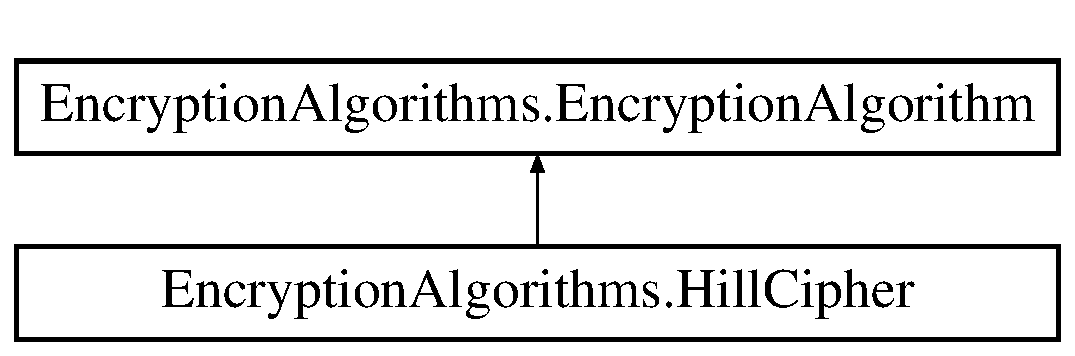
\includegraphics[height=2.000000cm]{classEncryptionAlgorithms_1_1HillCipher}
\end{center}
\end{figure}
\subsection*{Private Member Functions}
\begin{DoxyCompactItemize}
\item 
def \mbox{\hyperlink{classEncryptionAlgorithms_1_1HillCipher_adcc154da68ea72b40661bbc12315604f}{\+\_\+validate\+Key}} (self, key)
\begin{DoxyCompactList}\small\item\em Validates the key. \end{DoxyCompactList}\item 
def \mbox{\hyperlink{classEncryptionAlgorithms_1_1HillCipher_a3a9607e614402c2d7daa85d074b44a05}{\+\_\+validate\+Plain\+Text}} (self, text)
\begin{DoxyCompactList}\small\item\em validates the plain text. \end{DoxyCompactList}\item 
def \mbox{\hyperlink{classEncryptionAlgorithms_1_1HillCipher_ada1350994864531981e9d6d67f64e99c}{\+\_\+validate\+Cipher\+Text}} (self, text)
\begin{DoxyCompactList}\small\item\em validates the cipher text. \end{DoxyCompactList}\item 
def \mbox{\hyperlink{classEncryptionAlgorithms_1_1HillCipher_a68387a2463c5fc0d3753cf49a3c93d3b}{\+\_\+encrypt}} (self, key, text)
\begin{DoxyCompactList}\small\item\em Internal encryption function. \end{DoxyCompactList}\item 
def \mbox{\hyperlink{classEncryptionAlgorithms_1_1HillCipher_a35c4b5497e9a1a3e080dd8c4606f0003}{\+\_\+decrypt}} (self, key, text)
\begin{DoxyCompactList}\small\item\em Internal decryption function. \end{DoxyCompactList}\end{DoxyCompactItemize}
\subsection*{Additional Inherited Members}


\subsection{Detailed Description}
Extends \mbox{\hyperlink{classEncryptionAlgorithms_1_1EncryptionAlgorithm}{Encryption\+Algorithm}}. 

\subsection{Member Function Documentation}
\mbox{\Hypertarget{classEncryptionAlgorithms_1_1HillCipher_a35c4b5497e9a1a3e080dd8c4606f0003}\label{classEncryptionAlgorithms_1_1HillCipher_a35c4b5497e9a1a3e080dd8c4606f0003}} 
\index{Encryption\+Algorithms\+::\+Hill\+Cipher@{Encryption\+Algorithms\+::\+Hill\+Cipher}!\+\_\+decrypt@{\+\_\+decrypt}}
\index{\+\_\+decrypt@{\+\_\+decrypt}!Encryption\+Algorithms\+::\+Hill\+Cipher@{Encryption\+Algorithms\+::\+Hill\+Cipher}}
\subsubsection{\texorpdfstring{\+\_\+decrypt()}{\_decrypt()}}
{\footnotesize\ttfamily def Encryption\+Algorithms.\+Hill\+Cipher.\+\_\+decrypt (\begin{DoxyParamCaption}\item[{}]{self,  }\item[{}]{key,  }\item[{}]{text }\end{DoxyParamCaption})\hspace{0.3cm}{\ttfamily [private]}}



Internal decryption function. 

Splits the plaintext in blocks of length N(key is a matrix of Nx\+N). and concatenates dot products between the modular inverse of the key and each block.


\begin{DoxyParams}{Parameters}
{\em key} & \\
\hline
{\em text} & \\
\hline
\end{DoxyParams}
\begin{DoxyReturn}{Returns}

\end{DoxyReturn}
\mbox{\Hypertarget{classEncryptionAlgorithms_1_1HillCipher_a68387a2463c5fc0d3753cf49a3c93d3b}\label{classEncryptionAlgorithms_1_1HillCipher_a68387a2463c5fc0d3753cf49a3c93d3b}} 
\index{Encryption\+Algorithms\+::\+Hill\+Cipher@{Encryption\+Algorithms\+::\+Hill\+Cipher}!\+\_\+encrypt@{\+\_\+encrypt}}
\index{\+\_\+encrypt@{\+\_\+encrypt}!Encryption\+Algorithms\+::\+Hill\+Cipher@{Encryption\+Algorithms\+::\+Hill\+Cipher}}
\subsubsection{\texorpdfstring{\+\_\+encrypt()}{\_encrypt()}}
{\footnotesize\ttfamily def Encryption\+Algorithms.\+Hill\+Cipher.\+\_\+encrypt (\begin{DoxyParamCaption}\item[{}]{self,  }\item[{}]{key,  }\item[{}]{text }\end{DoxyParamCaption})\hspace{0.3cm}{\ttfamily [private]}}



Internal encryption function. 

Splits the plaintext in blocks of length N(key is a matrix of Nx\+N). and concatenates dot products between key and each block.


\begin{DoxyParams}{Parameters}
{\em key} & \\
\hline
{\em text} & \\
\hline
\end{DoxyParams}
\begin{DoxyReturn}{Returns}

\end{DoxyReturn}
\mbox{\Hypertarget{classEncryptionAlgorithms_1_1HillCipher_ada1350994864531981e9d6d67f64e99c}\label{classEncryptionAlgorithms_1_1HillCipher_ada1350994864531981e9d6d67f64e99c}} 
\index{Encryption\+Algorithms\+::\+Hill\+Cipher@{Encryption\+Algorithms\+::\+Hill\+Cipher}!\+\_\+validate\+Cipher\+Text@{\+\_\+validate\+Cipher\+Text}}
\index{\+\_\+validate\+Cipher\+Text@{\+\_\+validate\+Cipher\+Text}!Encryption\+Algorithms\+::\+Hill\+Cipher@{Encryption\+Algorithms\+::\+Hill\+Cipher}}
\subsubsection{\texorpdfstring{\+\_\+validate\+Cipher\+Text()}{\_validateCipherText()}}
{\footnotesize\ttfamily def Encryption\+Algorithms.\+Hill\+Cipher.\+\_\+validate\+Cipher\+Text (\begin{DoxyParamCaption}\item[{}]{self,  }\item[{}]{text }\end{DoxyParamCaption})\hspace{0.3cm}{\ttfamily [private]}}



validates the cipher text. 

Throws Validation\+Exception. Ciphertext has to contain only characters from the uppercase(alphabet).


\begin{DoxyParams}{Parameters}
{\em text} & \\
\hline
\end{DoxyParams}
\begin{DoxyReturn}{Returns}

\end{DoxyReturn}
\mbox{\Hypertarget{classEncryptionAlgorithms_1_1HillCipher_adcc154da68ea72b40661bbc12315604f}\label{classEncryptionAlgorithms_1_1HillCipher_adcc154da68ea72b40661bbc12315604f}} 
\index{Encryption\+Algorithms\+::\+Hill\+Cipher@{Encryption\+Algorithms\+::\+Hill\+Cipher}!\+\_\+validate\+Key@{\+\_\+validate\+Key}}
\index{\+\_\+validate\+Key@{\+\_\+validate\+Key}!Encryption\+Algorithms\+::\+Hill\+Cipher@{Encryption\+Algorithms\+::\+Hill\+Cipher}}
\subsubsection{\texorpdfstring{\+\_\+validate\+Key()}{\_validateKey()}}
{\footnotesize\ttfamily def Encryption\+Algorithms.\+Hill\+Cipher.\+\_\+validate\+Key (\begin{DoxyParamCaption}\item[{}]{self,  }\item[{}]{key }\end{DoxyParamCaption})\hspace{0.3cm}{\ttfamily [private]}}



Validates the key. 

Throws Validation\+Exception. Key is a square matrix of integers given as a list of nxn elements. Key has to be invertible and gcd(det(key), len(alphabet)) has to be 1. 
\begin{DoxyParams}{Parameters}
{\em key} & \\
\hline
\end{DoxyParams}
\begin{DoxyReturn}{Returns}

\end{DoxyReturn}
\mbox{\Hypertarget{classEncryptionAlgorithms_1_1HillCipher_a3a9607e614402c2d7daa85d074b44a05}\label{classEncryptionAlgorithms_1_1HillCipher_a3a9607e614402c2d7daa85d074b44a05}} 
\index{Encryption\+Algorithms\+::\+Hill\+Cipher@{Encryption\+Algorithms\+::\+Hill\+Cipher}!\+\_\+validate\+Plain\+Text@{\+\_\+validate\+Plain\+Text}}
\index{\+\_\+validate\+Plain\+Text@{\+\_\+validate\+Plain\+Text}!Encryption\+Algorithms\+::\+Hill\+Cipher@{Encryption\+Algorithms\+::\+Hill\+Cipher}}
\subsubsection{\texorpdfstring{\+\_\+validate\+Plain\+Text()}{\_validatePlainText()}}
{\footnotesize\ttfamily def Encryption\+Algorithms.\+Hill\+Cipher.\+\_\+validate\+Plain\+Text (\begin{DoxyParamCaption}\item[{}]{self,  }\item[{}]{text }\end{DoxyParamCaption})\hspace{0.3cm}{\ttfamily [private]}}



validates the plain text. 

Throws Validation\+Exception. Plaintext has to contain only characters from the alphabet.


\begin{DoxyParams}{Parameters}
{\em text} & \\
\hline
\end{DoxyParams}
\begin{DoxyReturn}{Returns}

\end{DoxyReturn}


The documentation for this class was generated from the following file\+:\begin{DoxyCompactItemize}
\item 
\mbox{\hyperlink{EncryptionAlgorithms_8py}{Encryption\+Algorithms.\+py}}\end{DoxyCompactItemize}

\hypertarget{classEncryptionAlgorithms_1_1PermutationCipher}{}\section{Encryption\+Algorithms.\+Permutation\+Cipher Class Reference}
\label{classEncryptionAlgorithms_1_1PermutationCipher}\index{Encryption\+Algorithms.\+Permutation\+Cipher@{Encryption\+Algorithms.\+Permutation\+Cipher}}
Inheritance diagram for Encryption\+Algorithms.\+Permutation\+Cipher\+:\begin{figure}[H]
\begin{center}
\leavevmode
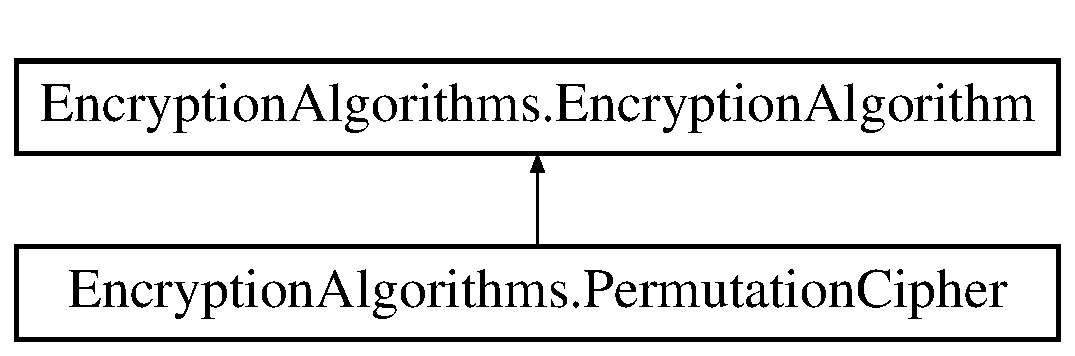
\includegraphics[height=2.000000cm]{classEncryptionAlgorithms_1_1PermutationCipher}
\end{center}
\end{figure}
\subsection*{Private Member Functions}
\begin{DoxyCompactItemize}
\item 
def \mbox{\hyperlink{classEncryptionAlgorithms_1_1PermutationCipher_acb25f849a94ae3e4e09c89538161d5df}{\+\_\+validate\+Key}} (self, key)
\item 
def \mbox{\hyperlink{classEncryptionAlgorithms_1_1PermutationCipher_a945832a0811988d4c15ef05923c26b6c}{\+\_\+validate\+Plain\+Text}} (self, text)
\item 
def \mbox{\hyperlink{classEncryptionAlgorithms_1_1PermutationCipher_a223a8ae8f5541420088a0b50a738c8ea}{\+\_\+validate\+Cipher\+Text}} (self, text)
\item 
def \mbox{\hyperlink{classEncryptionAlgorithms_1_1PermutationCipher_a81b8d8bcde87b89858849a48c9228351}{\+\_\+encrypt}} (self, key, text)
\item 
def \mbox{\hyperlink{classEncryptionAlgorithms_1_1PermutationCipher_a9cc459cdb613ceea51389446036c4814}{\+\_\+decrypt}} (self, key, text)
\end{DoxyCompactItemize}
\subsection*{Additional Inherited Members}


\subsection{Member Function Documentation}
\mbox{\Hypertarget{classEncryptionAlgorithms_1_1PermutationCipher_a9cc459cdb613ceea51389446036c4814}\label{classEncryptionAlgorithms_1_1PermutationCipher_a9cc459cdb613ceea51389446036c4814}} 
\index{Encryption\+Algorithms\+::\+Permutation\+Cipher@{Encryption\+Algorithms\+::\+Permutation\+Cipher}!\+\_\+decrypt@{\+\_\+decrypt}}
\index{\+\_\+decrypt@{\+\_\+decrypt}!Encryption\+Algorithms\+::\+Permutation\+Cipher@{Encryption\+Algorithms\+::\+Permutation\+Cipher}}
\subsubsection{\texorpdfstring{\+\_\+decrypt()}{\_decrypt()}}
{\footnotesize\ttfamily def Encryption\+Algorithms.\+Permutation\+Cipher.\+\_\+decrypt (\begin{DoxyParamCaption}\item[{}]{self,  }\item[{}]{key,  }\item[{}]{text }\end{DoxyParamCaption})\hspace{0.3cm}{\ttfamily [private]}}

\mbox{\Hypertarget{classEncryptionAlgorithms_1_1PermutationCipher_a81b8d8bcde87b89858849a48c9228351}\label{classEncryptionAlgorithms_1_1PermutationCipher_a81b8d8bcde87b89858849a48c9228351}} 
\index{Encryption\+Algorithms\+::\+Permutation\+Cipher@{Encryption\+Algorithms\+::\+Permutation\+Cipher}!\+\_\+encrypt@{\+\_\+encrypt}}
\index{\+\_\+encrypt@{\+\_\+encrypt}!Encryption\+Algorithms\+::\+Permutation\+Cipher@{Encryption\+Algorithms\+::\+Permutation\+Cipher}}
\subsubsection{\texorpdfstring{\+\_\+encrypt()}{\_encrypt()}}
{\footnotesize\ttfamily def Encryption\+Algorithms.\+Permutation\+Cipher.\+\_\+encrypt (\begin{DoxyParamCaption}\item[{}]{self,  }\item[{}]{key,  }\item[{}]{text }\end{DoxyParamCaption})\hspace{0.3cm}{\ttfamily [private]}}

\mbox{\Hypertarget{classEncryptionAlgorithms_1_1PermutationCipher_a223a8ae8f5541420088a0b50a738c8ea}\label{classEncryptionAlgorithms_1_1PermutationCipher_a223a8ae8f5541420088a0b50a738c8ea}} 
\index{Encryption\+Algorithms\+::\+Permutation\+Cipher@{Encryption\+Algorithms\+::\+Permutation\+Cipher}!\+\_\+validate\+Cipher\+Text@{\+\_\+validate\+Cipher\+Text}}
\index{\+\_\+validate\+Cipher\+Text@{\+\_\+validate\+Cipher\+Text}!Encryption\+Algorithms\+::\+Permutation\+Cipher@{Encryption\+Algorithms\+::\+Permutation\+Cipher}}
\subsubsection{\texorpdfstring{\+\_\+validate\+Cipher\+Text()}{\_validateCipherText()}}
{\footnotesize\ttfamily def Encryption\+Algorithms.\+Permutation\+Cipher.\+\_\+validate\+Cipher\+Text (\begin{DoxyParamCaption}\item[{}]{self,  }\item[{}]{text }\end{DoxyParamCaption})\hspace{0.3cm}{\ttfamily [private]}}

\mbox{\Hypertarget{classEncryptionAlgorithms_1_1PermutationCipher_acb25f849a94ae3e4e09c89538161d5df}\label{classEncryptionAlgorithms_1_1PermutationCipher_acb25f849a94ae3e4e09c89538161d5df}} 
\index{Encryption\+Algorithms\+::\+Permutation\+Cipher@{Encryption\+Algorithms\+::\+Permutation\+Cipher}!\+\_\+validate\+Key@{\+\_\+validate\+Key}}
\index{\+\_\+validate\+Key@{\+\_\+validate\+Key}!Encryption\+Algorithms\+::\+Permutation\+Cipher@{Encryption\+Algorithms\+::\+Permutation\+Cipher}}
\subsubsection{\texorpdfstring{\+\_\+validate\+Key()}{\_validateKey()}}
{\footnotesize\ttfamily def Encryption\+Algorithms.\+Permutation\+Cipher.\+\_\+validate\+Key (\begin{DoxyParamCaption}\item[{}]{self,  }\item[{}]{key }\end{DoxyParamCaption})\hspace{0.3cm}{\ttfamily [private]}}

\mbox{\Hypertarget{classEncryptionAlgorithms_1_1PermutationCipher_a945832a0811988d4c15ef05923c26b6c}\label{classEncryptionAlgorithms_1_1PermutationCipher_a945832a0811988d4c15ef05923c26b6c}} 
\index{Encryption\+Algorithms\+::\+Permutation\+Cipher@{Encryption\+Algorithms\+::\+Permutation\+Cipher}!\+\_\+validate\+Plain\+Text@{\+\_\+validate\+Plain\+Text}}
\index{\+\_\+validate\+Plain\+Text@{\+\_\+validate\+Plain\+Text}!Encryption\+Algorithms\+::\+Permutation\+Cipher@{Encryption\+Algorithms\+::\+Permutation\+Cipher}}
\subsubsection{\texorpdfstring{\+\_\+validate\+Plain\+Text()}{\_validatePlainText()}}
{\footnotesize\ttfamily def Encryption\+Algorithms.\+Permutation\+Cipher.\+\_\+validate\+Plain\+Text (\begin{DoxyParamCaption}\item[{}]{self,  }\item[{}]{text }\end{DoxyParamCaption})\hspace{0.3cm}{\ttfamily [private]}}



The documentation for this class was generated from the following file\+:\begin{DoxyCompactItemize}
\item 
\mbox{\hyperlink{EncryptionAlgorithms_8py}{Encryption\+Algorithms.\+py}}\end{DoxyCompactItemize}

\hypertarget{classEncryptionAlgorithms_1_1SubstitutionCipher}{}\section{Encryption\+Algorithms.\+Substitution\+Cipher Class Reference}
\label{classEncryptionAlgorithms_1_1SubstitutionCipher}\index{Encryption\+Algorithms.\+Substitution\+Cipher@{Encryption\+Algorithms.\+Substitution\+Cipher}}


Extends \mbox{\hyperlink{classEncryptionAlgorithms_1_1EncryptionAlgorithm}{Encryption\+Algorithm}}.  


Inheritance diagram for Encryption\+Algorithms.\+Substitution\+Cipher\+:\begin{figure}[H]
\begin{center}
\leavevmode
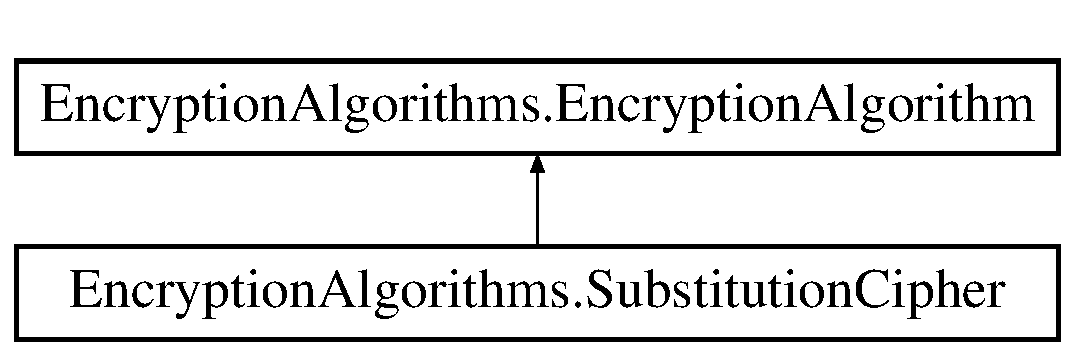
\includegraphics[height=2.000000cm]{classEncryptionAlgorithms_1_1SubstitutionCipher}
\end{center}
\end{figure}
\subsection*{Public Member Functions}
\begin{DoxyCompactItemize}
\item 
def \mbox{\hyperlink{classEncryptionAlgorithms_1_1SubstitutionCipher_ac8d0e10409c6dd0ac7cbb7bf94f4f2bd}{decrypt}} (self, key, text)
\begin{DoxyCompactList}\small\item\em Overload on decrypth method. \end{DoxyCompactList}\end{DoxyCompactItemize}
\subsection*{Private Member Functions}
\begin{DoxyCompactItemize}
\item 
def \mbox{\hyperlink{classEncryptionAlgorithms_1_1SubstitutionCipher_a3ec601adf1b00d35706c42afac3d194e}{\+\_\+validate\+Key}} (self, key)
\begin{DoxyCompactList}\small\item\em validates the key. \end{DoxyCompactList}\item 
def \mbox{\hyperlink{classEncryptionAlgorithms_1_1SubstitutionCipher_a0dc91efdbee882c4b1e1fbcb2c6a8709}{\+\_\+validate\+Plain\+Text}} (self, text)
\begin{DoxyCompactList}\small\item\em validates the plain text. \end{DoxyCompactList}\item 
def \mbox{\hyperlink{classEncryptionAlgorithms_1_1SubstitutionCipher_af8725d1344b2f6dd47f1e3303ab049eb}{\+\_\+validate\+Cipher\+Text}} (self, key, text)
\begin{DoxyCompactList}\small\item\em validates the cipher text. \end{DoxyCompactList}\item 
def \mbox{\hyperlink{classEncryptionAlgorithms_1_1SubstitutionCipher_ae877efaf2ea953c760770d92d719517a}{\+\_\+encrypt}} (self, key, text)
\begin{DoxyCompactList}\small\item\em Internal encryption function. \end{DoxyCompactList}\item 
def \mbox{\hyperlink{classEncryptionAlgorithms_1_1SubstitutionCipher_ac7b54cd92d6d1c1cb5a90a9c603d50c1}{\+\_\+decrypt}} (self, key, text)
\begin{DoxyCompactList}\small\item\em Internal decryption function. \end{DoxyCompactList}\end{DoxyCompactItemize}
\subsection*{Additional Inherited Members}


\subsection{Detailed Description}
Extends \mbox{\hyperlink{classEncryptionAlgorithms_1_1EncryptionAlgorithm}{Encryption\+Algorithm}}. 

\subsection{Member Function Documentation}
\mbox{\Hypertarget{classEncryptionAlgorithms_1_1SubstitutionCipher_ac7b54cd92d6d1c1cb5a90a9c603d50c1}\label{classEncryptionAlgorithms_1_1SubstitutionCipher_ac7b54cd92d6d1c1cb5a90a9c603d50c1}} 
\index{Encryption\+Algorithms\+::\+Substitution\+Cipher@{Encryption\+Algorithms\+::\+Substitution\+Cipher}!\+\_\+decrypt@{\+\_\+decrypt}}
\index{\+\_\+decrypt@{\+\_\+decrypt}!Encryption\+Algorithms\+::\+Substitution\+Cipher@{Encryption\+Algorithms\+::\+Substitution\+Cipher}}
\subsubsection{\texorpdfstring{\+\_\+decrypt()}{\_decrypt()}}
{\footnotesize\ttfamily def Encryption\+Algorithms.\+Substitution\+Cipher.\+\_\+decrypt (\begin{DoxyParamCaption}\item[{}]{self,  }\item[{}]{key,  }\item[{}]{text }\end{DoxyParamCaption})\hspace{0.3cm}{\ttfamily [private]}}



Internal decryption function. 

Substitutes each character in the ciphertext with the corresponding character in the plaintext.


\begin{DoxyParams}{Parameters}
{\em key} & \\
\hline
{\em text} & \\
\hline
\end{DoxyParams}
\begin{DoxyReturn}{Returns}
Decrypted text 
\end{DoxyReturn}
\mbox{\Hypertarget{classEncryptionAlgorithms_1_1SubstitutionCipher_ae877efaf2ea953c760770d92d719517a}\label{classEncryptionAlgorithms_1_1SubstitutionCipher_ae877efaf2ea953c760770d92d719517a}} 
\index{Encryption\+Algorithms\+::\+Substitution\+Cipher@{Encryption\+Algorithms\+::\+Substitution\+Cipher}!\+\_\+encrypt@{\+\_\+encrypt}}
\index{\+\_\+encrypt@{\+\_\+encrypt}!Encryption\+Algorithms\+::\+Substitution\+Cipher@{Encryption\+Algorithms\+::\+Substitution\+Cipher}}
\subsubsection{\texorpdfstring{\+\_\+encrypt()}{\_encrypt()}}
{\footnotesize\ttfamily def Encryption\+Algorithms.\+Substitution\+Cipher.\+\_\+encrypt (\begin{DoxyParamCaption}\item[{}]{self,  }\item[{}]{key,  }\item[{}]{text }\end{DoxyParamCaption})\hspace{0.3cm}{\ttfamily [private]}}



Internal encryption function. 

Substitutes each character in the plaintext with the corresponding character in the ciphertext.


\begin{DoxyParams}{Parameters}
{\em key} & \\
\hline
{\em text} & \\
\hline
\end{DoxyParams}
\begin{DoxyReturn}{Returns}
Encrypted text 
\end{DoxyReturn}
\mbox{\Hypertarget{classEncryptionAlgorithms_1_1SubstitutionCipher_af8725d1344b2f6dd47f1e3303ab049eb}\label{classEncryptionAlgorithms_1_1SubstitutionCipher_af8725d1344b2f6dd47f1e3303ab049eb}} 
\index{Encryption\+Algorithms\+::\+Substitution\+Cipher@{Encryption\+Algorithms\+::\+Substitution\+Cipher}!\+\_\+validate\+Cipher\+Text@{\+\_\+validate\+Cipher\+Text}}
\index{\+\_\+validate\+Cipher\+Text@{\+\_\+validate\+Cipher\+Text}!Encryption\+Algorithms\+::\+Substitution\+Cipher@{Encryption\+Algorithms\+::\+Substitution\+Cipher}}
\subsubsection{\texorpdfstring{\+\_\+validate\+Cipher\+Text()}{\_validateCipherText()}}
{\footnotesize\ttfamily def Encryption\+Algorithms.\+Substitution\+Cipher.\+\_\+validate\+Cipher\+Text (\begin{DoxyParamCaption}\item[{}]{self,  }\item[{}]{key,  }\item[{}]{text }\end{DoxyParamCaption})\hspace{0.3cm}{\ttfamily [private]}}



validates the cipher text. 

Throws Validation\+Exception. Ciphertext has to contain only characters from the uppercase(alphabet).


\begin{DoxyParams}{Parameters}
{\em text} & \\
\hline
\end{DoxyParams}
\begin{DoxyReturn}{Returns}

\end{DoxyReturn}
\mbox{\Hypertarget{classEncryptionAlgorithms_1_1SubstitutionCipher_a3ec601adf1b00d35706c42afac3d194e}\label{classEncryptionAlgorithms_1_1SubstitutionCipher_a3ec601adf1b00d35706c42afac3d194e}} 
\index{Encryption\+Algorithms\+::\+Substitution\+Cipher@{Encryption\+Algorithms\+::\+Substitution\+Cipher}!\+\_\+validate\+Key@{\+\_\+validate\+Key}}
\index{\+\_\+validate\+Key@{\+\_\+validate\+Key}!Encryption\+Algorithms\+::\+Substitution\+Cipher@{Encryption\+Algorithms\+::\+Substitution\+Cipher}}
\subsubsection{\texorpdfstring{\+\_\+validate\+Key()}{\_validateKey()}}
{\footnotesize\ttfamily def Encryption\+Algorithms.\+Substitution\+Cipher.\+\_\+validate\+Key (\begin{DoxyParamCaption}\item[{}]{self,  }\item[{}]{key }\end{DoxyParamCaption})\hspace{0.3cm}{\ttfamily [private]}}



validates the key. 

Throws Validation\+Exception. Key has to be a string with set properties and equal of length with the alphabet.


\begin{DoxyParams}{Parameters}
{\em key} & \\
\hline
\end{DoxyParams}
\begin{DoxyReturn}{Returns}

\end{DoxyReturn}
\mbox{\Hypertarget{classEncryptionAlgorithms_1_1SubstitutionCipher_a0dc91efdbee882c4b1e1fbcb2c6a8709}\label{classEncryptionAlgorithms_1_1SubstitutionCipher_a0dc91efdbee882c4b1e1fbcb2c6a8709}} 
\index{Encryption\+Algorithms\+::\+Substitution\+Cipher@{Encryption\+Algorithms\+::\+Substitution\+Cipher}!\+\_\+validate\+Plain\+Text@{\+\_\+validate\+Plain\+Text}}
\index{\+\_\+validate\+Plain\+Text@{\+\_\+validate\+Plain\+Text}!Encryption\+Algorithms\+::\+Substitution\+Cipher@{Encryption\+Algorithms\+::\+Substitution\+Cipher}}
\subsubsection{\texorpdfstring{\+\_\+validate\+Plain\+Text()}{\_validatePlainText()}}
{\footnotesize\ttfamily def Encryption\+Algorithms.\+Substitution\+Cipher.\+\_\+validate\+Plain\+Text (\begin{DoxyParamCaption}\item[{}]{self,  }\item[{}]{text }\end{DoxyParamCaption})\hspace{0.3cm}{\ttfamily [private]}}



validates the plain text. 

Throws Validation\+Exception. Plaintext has to contain only characters from the alphabet.


\begin{DoxyParams}{Parameters}
{\em text} & \\
\hline
\end{DoxyParams}
\begin{DoxyReturn}{Returns}

\end{DoxyReturn}
\mbox{\Hypertarget{classEncryptionAlgorithms_1_1SubstitutionCipher_ac8d0e10409c6dd0ac7cbb7bf94f4f2bd}\label{classEncryptionAlgorithms_1_1SubstitutionCipher_ac8d0e10409c6dd0ac7cbb7bf94f4f2bd}} 
\index{Encryption\+Algorithms\+::\+Substitution\+Cipher@{Encryption\+Algorithms\+::\+Substitution\+Cipher}!decrypt@{decrypt}}
\index{decrypt@{decrypt}!Encryption\+Algorithms\+::\+Substitution\+Cipher@{Encryption\+Algorithms\+::\+Substitution\+Cipher}}
\subsubsection{\texorpdfstring{decrypt()}{decrypt()}}
{\footnotesize\ttfamily def Encryption\+Algorithms.\+Substitution\+Cipher.\+decrypt (\begin{DoxyParamCaption}\item[{}]{self,  }\item[{}]{key,  }\item[{}]{text }\end{DoxyParamCaption})}



Overload on decrypth method. 

Overload needed because ciphertext validation has to include the key.


\begin{DoxyParams}{Parameters}
{\em key} & \\
\hline
{\em text} & \\
\hline
\end{DoxyParams}
\begin{DoxyReturn}{Returns}
Decrypted text 
\end{DoxyReturn}


The documentation for this class was generated from the following file\+:\begin{DoxyCompactItemize}
\item 
\mbox{\hyperlink{EncryptionAlgorithms_8py}{Encryption\+Algorithms.\+py}}\end{DoxyCompactItemize}

\hypertarget{classExceptions_1_1ValidationException}{}\section{Exceptions.\+Validation\+Exception Class Reference}
\label{classExceptions_1_1ValidationException}\index{Exceptions.\+Validation\+Exception@{Exceptions.\+Validation\+Exception}}
Inheritance diagram for Exceptions.\+Validation\+Exception\+:\begin{figure}[H]
\begin{center}
\leavevmode
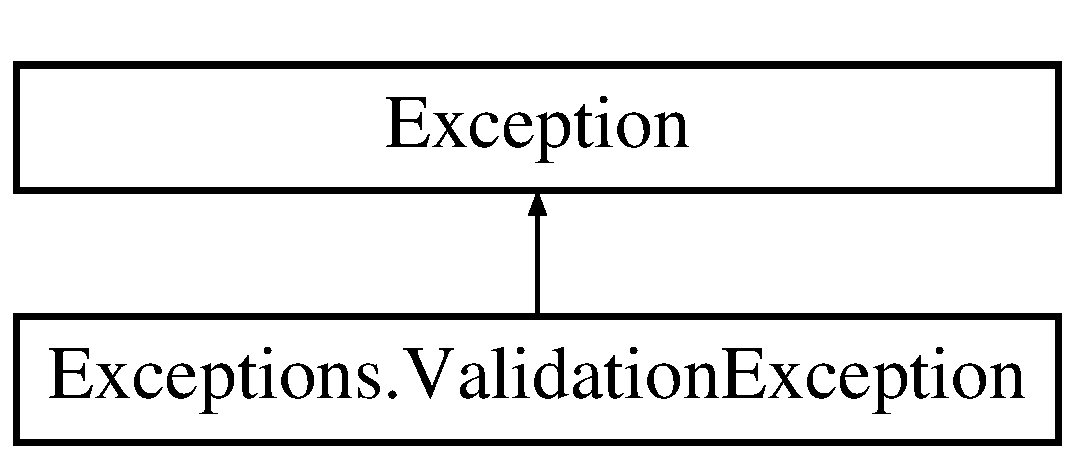
\includegraphics[height=2.000000cm]{classExceptions_1_1ValidationException}
\end{center}
\end{figure}


The documentation for this class was generated from the following file\+:\begin{DoxyCompactItemize}
\item 
\mbox{\hyperlink{Exceptions_8py}{Exceptions.\+py}}\end{DoxyCompactItemize}

\chapter{File Documentation}
\hypertarget{appjar__test_8py}{}\section{appjar\+\_\+test.\+py File Reference}
\label{appjar__test_8py}\index{appjar\+\_\+test.\+py@{appjar\+\_\+test.\+py}}
\subsection*{Namespaces}
\begin{DoxyCompactItemize}
\item 
 \mbox{\hyperlink{namespaceappjar__test}{appjar\+\_\+test}}
\end{DoxyCompactItemize}
\subsection*{Functions}
\begin{DoxyCompactItemize}
\item 
def \mbox{\hyperlink{namespaceappjar__test_a35ead9b75f3a80c900d90925d6aacf58}{appjar\+\_\+test.\+helpfun}} (app, cipher)
\item 
def \mbox{\hyperlink{namespaceappjar__test_a6abeaf134dae6285b648ef0e81159506}{appjar\+\_\+test.\+get\+Cipher}} (cipher, alphabet)
\item 
def \mbox{\hyperlink{namespaceappjar__test_a13cd64e5fb029fcee4ed6e61fe859344}{appjar\+\_\+test.\+get\+Key}} (cipher, keytext)
\item 
def \mbox{\hyperlink{namespaceappjar__test_a3b7395e7f8f122d03a183d0faa0fa494}{appjar\+\_\+test.\+encrypt}} (app, decrypt\+\_\+bool=False)
\end{DoxyCompactItemize}
\subsection*{Variables}
\begin{DoxyCompactItemize}
\item 
list \mbox{\hyperlink{namespaceappjar__test_aeaee605feadc2cd9b1dfaa00166e8dc2}{appjar\+\_\+test.\+ciphers}} = \mbox{[}\char`\"{}caesar\char`\"{}, \char`\"{}substitution\char`\"{}, \char`\"{}affine\char`\"{}, \char`\"{}belaso\char`\"{}, \char`\"{}hill\char`\"{}, \char`\"{}permutation\char`\"{}\mbox{]}
\end{DoxyCompactItemize}

\hypertarget{EncryptionAlgorithms_8py}{}\section{Encryption\+Algorithms.\+py File Reference}
\label{EncryptionAlgorithms_8py}\index{Encryption\+Algorithms.\+py@{Encryption\+Algorithms.\+py}}
\subsection*{Classes}
\begin{DoxyCompactItemize}
\item 
class \mbox{\hyperlink{classEncryptionAlgorithms_1_1EncryptionAlgorithm}{Encryption\+Algorithms.\+Encryption\+Algorithm}}
\begin{DoxyCompactList}\small\item\em Base encryption algorigm class, defines the A\+PI. \end{DoxyCompactList}\item 
class \mbox{\hyperlink{classEncryptionAlgorithms_1_1CaesarCipher}{Encryption\+Algorithms.\+Caesar\+Cipher}}
\begin{DoxyCompactList}\small\item\em Implements the Caesar cipher, has all methods from \mbox{\hyperlink{classEncryptionAlgorithms_1_1EncryptionAlgorithm}{Encryption\+Algorithm}}. \end{DoxyCompactList}\item 
class \mbox{\hyperlink{classEncryptionAlgorithms_1_1SubstitutionCipher}{Encryption\+Algorithms.\+Substitution\+Cipher}}
\begin{DoxyCompactList}\small\item\em Extends \mbox{\hyperlink{classEncryptionAlgorithms_1_1EncryptionAlgorithm}{Encryption\+Algorithm}}. \end{DoxyCompactList}\item 
class \mbox{\hyperlink{classEncryptionAlgorithms_1_1AffineCipher}{Encryption\+Algorithms.\+Affine\+Cipher}}
\item 
class \mbox{\hyperlink{classEncryptionAlgorithms_1_1BelasoCipher}{Encryption\+Algorithms.\+Belaso\+Cipher}}
\item 
class \mbox{\hyperlink{classEncryptionAlgorithms_1_1HillCipher}{Encryption\+Algorithms.\+Hill\+Cipher}}
\begin{DoxyCompactList}\small\item\em Extends \mbox{\hyperlink{classEncryptionAlgorithms_1_1EncryptionAlgorithm}{Encryption\+Algorithm}}. \end{DoxyCompactList}\item 
class \mbox{\hyperlink{classEncryptionAlgorithms_1_1PermutationCipher}{Encryption\+Algorithms.\+Permutation\+Cipher}}
\end{DoxyCompactItemize}
\subsection*{Namespaces}
\begin{DoxyCompactItemize}
\item 
 \mbox{\hyperlink{namespaceEncryptionAlgorithms}{Encryption\+Algorithms}}
\end{DoxyCompactItemize}
\subsection*{Functions}
\begin{DoxyCompactItemize}
\item 
def \mbox{\hyperlink{namespaceEncryptionAlgorithms_a579c44082c46469c685af4fa13b7087e}{Encryption\+Algorithms.\+\_\+gcd}} (a, b)
\begin{DoxyCompactList}\small\item\em Greatest common divisor between two positive integers. \end{DoxyCompactList}\item 
def \mbox{\hyperlink{namespaceEncryptionAlgorithms_ac6020cd3bf4adee2c1d7e325d0218630}{Encryption\+Algorithms.\+gcd}} (a, b)
\begin{DoxyCompactList}\small\item\em Greatest common divisor between two integer. \end{DoxyCompactList}\item 
def \mbox{\hyperlink{namespaceEncryptionAlgorithms_a054a518c18879771f989654ab7e2ae4e}{Encryption\+Algorithms.\+\_\+egcd}} (a, b)
\begin{DoxyCompactList}\small\item\em Extended greatest common divisor between two positive integers. \end{DoxyCompactList}\item 
def \mbox{\hyperlink{namespaceEncryptionAlgorithms_a8202b546cf0698eece91364d04351eac}{Encryption\+Algorithms.\+egcd}} (a, b)
\begin{DoxyCompactList}\small\item\em Extended greatest common divisor between two positive integers. \end{DoxyCompactList}\end{DoxyCompactItemize}

\hypertarget{Exceptions_8py}{}\section{Exceptions.\+py File Reference}
\label{Exceptions_8py}\index{Exceptions.\+py@{Exceptions.\+py}}
\subsection*{Classes}
\begin{DoxyCompactItemize}
\item 
class \mbox{\hyperlink{classExceptions_1_1ValidationException}{Exceptions.\+Validation\+Exception}}
\end{DoxyCompactItemize}
\subsection*{Namespaces}
\begin{DoxyCompactItemize}
\item 
 \mbox{\hyperlink{namespaceExceptions}{Exceptions}}
\end{DoxyCompactItemize}

%--- End generated contents ---

% Index
\backmatter
\newpage
\phantomsection
\clearemptydoublepage
\addcontentsline{toc}{chapter}{Index}
\printindex

\end{document}
